% Grounded Transport: A Proof-Relevant Rewriting Calculus for Lineage-Sensitive Systems
% Target: Logical Methods in Computer Science (LMCS).  DRAFT 2.
% Build: make   (uses the official lmcs.cls, downloaded from
%        https://lmcs.episciences.org/public/lmcs.cls; re-download before submission)
\documentclass{lmcs}

\usepackage{amssymb}
\usepackage{booktabs,array,tabularx,longtable,centernot}
\usetikzlibrary{arrows.meta,positioning,shapes.geometric}
\usepackage{hyperref}   % loaded here so that cleveref (which must follow it) works with lmcs.cls
\usepackage{xurl}
\usepackage[capitalise,noabbrev]{cleveref}

\emergencystretch=3em

% ---------- cross-reference names for LMCS environments ----------
\crefname{thm}{Theorem}{Theorems}
\crefname{lem}{Lemma}{Lemmas}
\crefname{prop}{Proposition}{Propositions}
\crefname{cor}{Corollary}{Corollaries}
\crefname{defi}{Definition}{Definitions}
\crefname{exa}{Example}{Examples}
\crefname{rem}{Remark}{Remarks}

% ---------- macros ----------
\DeclareUrlCommand\coq{\def\UrlFont{\ttfamily\small\upshape}}   % Coq identifiers (breakable)
\newcommand{\GTrans}{\mathsf{GTrans}}
\newcommand{\Cross}{\mathsf{Cross}}
\newcommand{\erase}{\mathsf{erase}}
\newcommand{\erased}{\mathsf{erased}}
\newcommand{\Prop}{\mathsf{Prop}}
\newcommand{\Type}{\mathsf{Type}}
\newcommand{\back}{\mathrm{back}}
\newcommand{\fwd}{\mathrm{fwd}}
\newcommand{\Cert}{\mathsf{Certified}}
\newcommand{\Refu}{\mathsf{Refuted}}
\newcommand{\Open}{\mathsf{Open}}
\newcommand{\Proper}{\mathsf{Proper}}
\newcommand{\GProper}{\mathsf{GroundedProper}}
\newcommand{\anc}{\mathrm{anc}}
\newcommand{\nat}{\mathbb{N}}
\newcommand{\bool}{\mathbb{B}}
\newcommand{\val}{\mathrm{val}}
\newcommand{\Adm}{\mathrm{Adm}}
\newcommand{\Tr}{\mathsf{Transportable}}
\newcommand{\weq}{\mathrel{\simeq}}
\newcolumntype{Y}{>{\raggedright\arraybackslash}X}

\begin{document}

\title[Grounded Transport]{Grounded Transport: A Proof-Relevant Rewriting Calculus for Lineage-Sensitive Systems}

\author[D.~Moore]{Duston Moore}
\address{Independent Researcher, Edmonton, Alberta, Canada}
\email{dhwcmoore@gmail.com}

\keywords{proof-relevant rewriting, transport, erasure, provenance and lineage, mechanised metatheory, Coq, certified decision procedures, extraction}
\ACMCCS{[{\bf Theory of computation}]: Logic---Logic and verification; Equational logic and rewriting; Type theory}

\begin{abstract}
\noindent
Ordinary rewriting records that one expression may replace another under an extensional relation.
In lineage-sensitive systems this is not always enough: whether a substitution is warranted may also depend on the process connecting the terms, on whether that process was independently grounded, on whether its evidence has been maintained through time, and on which obligations remain unresolved.
We introduce a directed, proof-relevant transport calculus in which this warrant is carried as extractable data.
Erasure, in two stages, recovers ordinary substitutability; we prove that erasure is sound, that it does not reflect grounding, and that distinct warrants can erase to the same judgement.
Contexts are treated at two levels: crossing-proper contexts preserve certified crossings, and certificate-proper contexts additionally preserve complete certificates and need an evidence lift; both compose and erase to ordinary \texttt{Proper} contexts.
Instantiated on grounded seams, the calculus recovers an earlier seam-transport theorem, separates structural naturality from preservation of grounding, and yields located obstructions to substitution.
Assessment is problem-indexed and three-valued (certified, refuted, open), retains every located failure, and treats missing evidence as unresolved rather than refuted.
A finite lineage audit is proved to reflect its specification, and its extraction issues kernel-checked certificates.
The development is mechanised in Coq; the main development is axiom-free, and one isolated, non-imported functional converse uses classical choice. Extraction to OCaml shows that certificates, lineage graphs and obstructions survive proof erasure, and differential testing, including a mutation study, compares the extracted audit with a handwritten one.
The calculus does not establish that declared records are complete or accurate; it makes precisely explicit what is being declared.
\end{abstract}

\maketitle

\section{Introduction}\label{sec:intro}

\subsection{The limitation of extensional rewriting}
Ordinary rewriting licenses substitution under a relation: if $x \mathrel{R} y$ and $C$ is a context that respects the relevant relations, then $C[x] \mathrel{R'} C[y]$. This is deliberately extensional. Once $x \mathrel{R} y$ has been established, the step normally does not retain how $x$ and $y$ were connected, which process produced the claimed agreement, whether one side was copied from the other, whether the evidence was independently grounded, whether the transformation has been maintained through time, or whether any obligation remains open.

For mathematical equality this forgetting is harmless, and it is the source of rewriting's power. For audited migrations, provenance-sensitive predicates, certified transformations and assurance arguments it is not always harmless: whether a substitution is \emph{warranted} can depend on exactly the information that a relational proof discards. We call the corresponding problem \emph{lineage-sensitive substitution}.

\subsection{A motivating separation}
Consider a dual-write migration. Two services record a status for each request, and an execution trace records what actually happened. On an ordinary request all three agree. On one exceptional request both services report success---because one copied the other---while the trace records failure. The two service records agree, so ordinary relational rewriting between them succeeds. If we ``repair'' the disagreement with the trace by defining the trace valuation to be the first service's value, every equation holds, but the ground now descends from the coordinate it was supposed to ground. The endpoint equation is true; its evidential warrant has failed. \Cref{sec:example} works this example out completely.

\subsection{The proposed solution}
We introduce \emph{grounded transport}. For a declared transport problem $c$, an inhabitant of $\GTrans_c(x,y) : \Type$ is not merely a proof that $x$ and $y$ are related: it carries the evidence by which transport is licensed, as data. Erasure recovers ordinary substitutability in two stages,
\[
\GTrans_c(x,y) \;\xrightarrow{\ \erase_1\ }\; \Cross_c(x,y) \;\xrightarrow{\ \erase_2\ }\; R(x,y),
\]
first forgetting certificates but keeping the directed crossing, then forgetting the crossing but keeping the relation. The central asymmetry is
\[
\GTrans_c(x,y) \Longrightarrow R(x,y), \qquad\text{but in general}\qquad R(x,y) \centernot\Longrightarrow \GTrans_c(x,y).
\]
Ordinary rewriting is thus the extensional image of the calculus, not something it abandons.

\subsection{Contributions}
Each contribution is a theorem about a mechanised calculus; named results refer to the Coq development (\cref{sec:mechanisation}).
\begin{enumerate}
\item \textbf{A grounded transport calculus} (\cref{sec:gt}): a directed, proof-relevant judgement carrying extractable seam, exhibition, lineage, coverage and record evidence; identity and composition; and algebraic laws stated modulo an explicit witness equivalence, since literal equality fails.
\item \textbf{Evidential erasure} (\cref{sec:erasure}): a two-stage erasure, its soundness, the induced preorder, a precise distinction between sound refinement and exact recovery, a proof that erasure does not reflect grounding, a proof that two distinct warrants for the same endpoints erase to the same judgement, and an observational obstruction showing why observational agreement cannot license lineage-sensitive substitution.
\item \textbf{Contexts at two levels} (\cref{sec:gt,sec:dynamic}): witness-mapping refinements of \texttt{Proper}: \emph{crossing-proper} contexts, which preserve certified crossings, and \emph{certificate-proper} contexts, which additionally preserve complete certificates and require an evidence lift. Both compose, certificate-proper implies crossing-proper implies \texttt{Proper}, and seam evolutions that preserve grounding on the image are crossing-proper but certificate-proper only under an evidence lift, which exists in one model and provably cannot in another.
\item \textbf{A canonical seam instance} (\cref{sec:seams}): recovery of an earlier seam-transport theorem from the generic calculus, with the observation that its conclusion needs only extensional agreement.
\item \textbf{Dynamic preservation and failure} (\cref{sec:dynamic}): a separation of structural naturality, valuation naturality, preservation of grounding, and coverage, and a model where ordinary rewriting remains valid while grounding is lost.
\item \textbf{Evidence-bearing assessment} (\cref{sec:assessment}): a problem-indexed three-valued semantics (certified, refuted, open) with located obstructions, soundness against a legacy transportability predicate, and cumulative failure reporting.
\item \textbf{Certified lineage checking} (\cref{sec:lineage}): a finite lineage audit with a proof of ancestor saturation and an \emph{unconditional} reflection theorem, whose extraction issues kernel-checked certificates, and a mechanised proof that pairwise accepted audits do not certify the outer coordinate pair (for a fixed graph and ground, L1 composes but L2 and L3 need not).
\item \textbf{Mechanised and tested evidence} (\cref{sec:mechanisation}): a Coq development whose main dependency closure is axiom-free (one isolated, non-imported functional converse uses classical choice), extraction showing that evidential data survive proof erasure, and differential testing---including a stratified test design and a mutation study---of the extracted audit against a handwritten one.
\end{enumerate}
We do not claim that equality, setoid rewriting, factorisation, or proof-relevant relations are new. The contribution is their integration into one calculus with the properties above, and the mechanised separation results.

\subsection{Scope and non-claims}
The calculus does \emph{not} prove that a declared lineage graph is complete; that raw evidence is accurate; that a state model adequately represents a concrete process; that an institutional authority is legitimate or competent; that every transport obligation is decidable; or that ordinary rewriting is unsound. The claim is that ordinary rewriting is \emph{evidentially incomplete} for some applications, and that this can be repaired without giving up its extensional image. The calculus makes explicit what is declared; it does not make declarations true.

\subsection{A note on motivation}
The design owes something to process philosophy: settled endpoints correspond to coordinate description, and a witness-bearing transition retains something of the production of that agreement. Nothing in the paper depends on that reading. The formal claim is only that endpoint agreement does not exhaust the evidence relevant to a transition (\cref{sec:whitehead}).

\section{A minimal separating example}\label{sec:example}

This section presents the counterexample in full, before any general definitions; it is reused in \cref{sec:erasure,sec:seams,sec:assessment}.

\subsection{The dual-write span}
Let $\Sigma = \{r_{\mathrm{ok}}, r_*\}$ be a set of requests and take $A = B = \Sigma$ with projections
\[
A \xleftarrow{\ \back\ } \Sigma \xrightarrow{\ \fwd\ } B, \qquad \back = \fwd = \mathrm{id}.
\]
Let both coordinate predicates be constantly true, $\Phi_A(\back(r)) = \Phi_B(\fwd(r)) = 1$. Then $\Phi_A \circ \back = \Phi_B \circ \fwd$: pairwise, \emph{extensional seam coherence} holds.

\subsection{The independently grounded valuation}
Let the seam carry its own valuation, exhibited from the execution trace:
\[
\Phi_\Sigma(r_{\mathrm{ok}}) = 1, \qquad \Phi_\Sigma(r_*) = 0.
\]
At $r_*$ we have $\Phi_A(\back(r_*)) = \Phi_B(\fwd(r_*)) = 1$ but $\Phi_\Sigma(r_*) = 0$: the coordinates agree with each other while disagreeing with the exhibited process.

\subsection{The copied alternative}
Defining instead $\widetilde{\Phi}_\Sigma = \Phi_A \circ \back$ satisfies all three equations. But its lineage descends from the very coordinate it is supposed to ground, so it fails the lineage requirement of \cref{sec:lineage}. Equational agreement, independent grounding and lineage warrant are thereby three separate things.

\subsection{Requirements}
The example demands that
(i) transport retain an \emph{exhibited crossing} (a seam element);
(ii) grounding refer to an \emph{independent seam valuation};
(iii) lineage be \emph{data}, not an erased proposition;
(iv) ordinary agreement be \emph{obtainable by erasure};
(v) failure report \emph{why} grounding was unavailable.
The question the calculus answers is: \emph{what must be retained so that the copied and independently grounded transports do not collapse into the same formal object?}

\section{Preliminaries}\label{sec:setting}

We fix only the notation needed later. The development is in Coq \cite{coq818}; we cite Coq identifiers in typewriter font so that each statement can be located in the artefact.

\paragraph{Relations and contexts.}
A \emph{directed relation} on a type $X$ is $R : X \to X \to \Prop$. We do not assume symmetry, since a migration, derivation or update may be valid from $x$ to $y$ without licensing reversal. A function $F : X \to Y$ is \emph{proper} for relations $R$ on $X$ and $S$ on $Y$ if $R(x,y)$ implies $S(Fx,Fy)$; this is the reading of Coq's \texttt{Proper} in generalised rewriting \cite{sozeau2009}. We use only this much of setoid rewriting: what a context must respect.

\paragraph{Proof relevance and extraction.}
The distinction that matters is between $R(x,y) : \Prop$ and $\GTrans(x,y) : \Type$. A type-valued judgement can have several distinguishable inhabitants connecting the same endpoints. In Coq, proof fields are erased on extraction, while data in \texttt{Type} remain; we place certificate \emph{data} in \texttt{Type} and the proofs that the data satisfy their specifications beside them. This is what lets extracted programs inspect evidence (\cref{sec:mechanisation}).

\paragraph{Lists, decidability, constructivity.}
$\mathsf{In}(x,l)$ is list membership; $l \mathbin{+\!\!+} l'$ is concatenation; $\mathsf{dedup}(l)$ removes duplicates. Except for one isolated theorem (\cref{sec:mechanisation}), all constructions are constructive.

\paragraph{The declared-evidence boundary.}
Throughout, two questions are kept apart: whether \emph{declared} records satisfy their stated conditions, which the kernel checks, and whether the declared records adequately represent the concrete world, which it cannot. The second is where the limits of \cref{sec:limitations} come from.

\section{Grounded transport}\label{sec:gt}

\subsection{Ordinary relations and grounded witnesses}\label{sec:witnesses}
An ordinary relational judgement $R(x,y) : \Prop$ says that $x$ and $y$ are related. A grounded judgement $\GTrans_c(x,y) : \Type$ is indexed by a declared \emph{transport problem} $c$ and its inhabitants carry inspectable evidence of why $x$ may be transported to $y$. We make this precise for the class of problems that includes the running example.

\begin{defi}[Transport problem]\label{def:problem}
A \emph{transport problem} $c$ consists of
\begin{itemize}
\item a span $A \xleftarrow{\back} \Sigma \xrightarrow{\fwd} B$ with Boolean valuations $\Phi_A$, $\Phi_B$ and a seam valuation $\Phi_\Sigma : \Sigma \to \bool$, and observation maps $M_A : A \to O_A$, $M_B : B \to O_B$;
\item a \emph{declared lineage record} $\ell$ (a finite structure, \cref{sec:lineage});
\item a type $\mathrm{Mnt}$ of maintenance evidence, a type $\mathrm{Mnt}^\bot$ of located maintenance failures, and a function $\mathrm{Mnt}^\bot \to \mathrm{Mnt} \to \bot$ saying that a failure refutes any evidence;
\item the same triple $(\mathrm{Aut}, \mathrm{Aut}^\bot, \mathrm{Aut}^\bot \to \mathrm{Aut} \to \bot)$ for authority evidence.
\end{itemize}
\end{defi}
The generic record fixes no institutional record format: maintenance and authority evidence are abstract types supplied by the application. Write $\Adm(M,\Phi) :\equiv \exists h.\ \Phi = h \circ M$ (admissibility of $\Phi$ with respect to observation $M$).

\begin{defi}[Certificates]\label{def:certs}
For a problem $c$ we have the following records, all in $\Type$.
\begin{enumerate}
\item An \emph{exhibition certificate} $\mathsf{Exh}(c)$: a record identifier; an injective assignment $\iota : \Sigma \to \nat$ of stable identifiers; a declared process; a type $\mathrm{Ret}$ of retained records with $\mathsf{retain} : \Sigma \to \mathrm{Ret}$ and $\mathsf{eval} : \mathrm{Ret} \to \bool$ such that $\Phi_\Sigma = \mathsf{eval} \circ \mathsf{retain}$ (the seam valuation is a function of what the record retains); a declared coverage interval; and a custodian identifier.
\item A \emph{lineage certificate} $\mathsf{Lin}$: a lineage graph $g$, a coverage record with its declared gaps, and an issued verdict, as \emph{data}; and proofs that $g$ is well-formed and satisfies L1--L3 (\cref{sec:lineage}), and that the gaps are empty.
\item A \emph{construction certificate} $\mathsf{Con}(c)$: an element $\sigma_0 \in \Sigma$; an $e \in \mathsf{Exh}(c)$; a $\lambda \in \mathsf{Lin}$ whose graph \emph{is} $\ell$; and the \emph{grounding equations} $\Phi_A(\back(r)) = \Phi_\Sigma(r)$ and $\Phi_B(\fwd(r)) = \Phi_\Sigma(r)$ for all $r$.
\item A \emph{certified transport} $\mathsf{Cert}(c) :\equiv \bigl(\Adm(M_A,\Phi_A) \wedge \Adm(M_B,\Phi_B)\bigr) \times \mathsf{Con}(c) \times \mathrm{Mnt} \times \mathrm{Aut}$.
\end{enumerate}
\end{defi}

\begin{defi}[States and grounded witnesses]\label{def:gtrans}
The \emph{states} of $c$ are $S_c :\equiv A + B$, with $\val(\mathsf{inl}\,a) = \Phi_A(a)$ and $\val(\mathsf{inr}\,b) = \Phi_B(b)$. The \emph{grounded witnesses} $\GTrans_c(s,t)$ are generated by
\begin{gather*}
\frac{}{\mathsf{id}_s : \GTrans_c(s,s)}\qquad
\frac{v : \GTrans_c(s,t) \quad w : \GTrans_c(t,u)}{v \cdot w : \GTrans_c(s,u)}\\[4pt]
\frac{r \in \Sigma \quad \kappa \in \mathsf{Cert}(c)}{\mathsf{step}(r,\kappa) : \GTrans_c(\mathsf{inl}\,\back(r),\ \mathsf{inr}\,\fwd(r))}
\end{gather*}
The \emph{crossing witnesses} $\Cross_c(s,t)$ are generated by the same rules except that $\mathsf{step}(r)$ requires only the two grounding equations at $r$ and no certificate.
\end{defi}

A witness is thus a directed path of crossings, each carrying a full certified transport. States are the disjoint union of the two coordinates; a crossing at $r$ leads from the $A$-side image $\back(r)$ to the $B$-side image $\fwd(r)$.

\paragraph{What survives extraction.}
The data-bearing components are: the seam element and its inhabitant; the exhibition record identifier, seam identifiers, process, retained-record function and evaluator, coverage interval and custodian; the lineage graph, coverage record with its gaps, and issued verdict; and the maintenance and authority evidence (to the extent the application supplies them in $\Type$). The proofs that these records satisfy their specifications---injectivity, factorisation, well-formedness, L1--L3, the grounding equations---certify the data but are erased.

\subsection{Why assessment is problem-indexed}\label{sec:indexed}
Two things must be kept apart: formal reflexivity of the transport relation, and the assessment of a proposed concrete transport problem.
\begin{quote}
\emph{Relational reflexivity is a property of the formal rewriting structure. It is not a certificate for every concrete process whose endpoints happen to be equal.}
\end{quote}
The identity witness $\mathsf{id}_s$ needs no certificate, so a judgement ``$s$ may be transported to $s$'' is always available formally. Yet a proposed \emph{process} that leaves a state representationally unchanged may have altered its provenance, calibration or authority; a pair-indexed assessment $\Refu(x,x)$ would contradict formal reflexivity, whereas a problem-indexed assessment can reject a proposed concrete process from $x$ to $x$ without doing so. Assessments (\cref{sec:assessment}) are therefore indexed by a transport \emph{problem}, and pair-level witnesses are \emph{derived} from a certified assessment.

\subsection{Identity and composition}\label{sec:laws}
Abstracting what all instances share gives:
\begin{defi}[Transport structure]\label{def:structure}
A \emph{transport structure} $G$ for a relation $R$ on $X$ is a family $\GTrans_G : X \to X \to \Type$ with an identity $\mathsf{id}_x : \GTrans_G(x,x)$, a composition $\GTrans_G(x,y) \to \GTrans_G(y,z) \to \GTrans_G(x,z)$, and a soundness map $\GTrans_G(x,y) \to R(x,y)$.
\end{defi}
$\GTrans_c$ is a transport structure for $R_c(s,t) :\equiv \val(s) = \val(t)$ (soundness is \cref{thm:soundness}), and so is $\Cross_c$.

\begin{thm}[Grounded reflexivity and composition]\label{thm:refl}
For every transport structure, $\mathsf{id}_x : \GTrans_G(x,x)$ and $\GTrans_G(x,y) \to \GTrans_G(y,z) \to \GTrans_G(x,z)$. In particular both hold for $\GTrans_c$, with $\mathsf{id}_s$ and $v \cdot w$. \emph{(Coq: \coq{grounded_transport_refl}, \coq{grounded_transport_compose}; mechanised, immediate from the definition.)}
\end{thm}

\paragraph{Algebraic laws.}
$\GTrans_c$ is a \emph{free} structure, so identity and associativity do not hold by literal equality: $\mathsf{id} \cdot w$ is not syntactically $w$. We therefore state them modulo an explicit equivalence. Let $\mathsf{crossings}(w)$ be the list of pairs $(r,\kappa)$ occurring in $w$, defined by $\mathsf{crossings}(\mathsf{id}) = [\,]$, $\mathsf{crossings}(\mathsf{step}(r,\kappa)) = [(r,\kappa)]$, and $\mathsf{crossings}(v \cdot w) = \mathsf{crossings}(v) \mathbin{+\!\!+} \mathsf{crossings}(w)$. Define
\[
w_1 \weq w_2 \;:\Longleftrightarrow\; \mathsf{crossings}(w_1) = \mathsf{crossings}(w_2).
\]
This forgets bracketing and identity padding and \emph{nothing else}: every seam element and every certificate is compared, and the comparison is by (dependent) equality.

\begin{thm}[Witness algebra]\label{thm:algebra}
$\weq$ is an equivalence relation on $\GTrans_c(s,t)$; composition respects it ($v \weq v'$ and $w \weq w'$ imply $v \cdot w \weq v' \cdot w'$); and
\[
\mathsf{id} \cdot w \weq w, \qquad w \cdot \mathsf{id} \weq w, \qquad (w_1 \cdot w_2) \cdot w_3 \weq w_1 \cdot (w_2 \cdot w_3).
\]
Moreover $w_1 \weq w_2$ implies that $w_1$ and $w_2$ have the same extractable summary (\cref{sec:multiplicity}). \emph{(Coq: \coq{WEquiv_id_left}, \coq{WEquiv_id_right}, \coq{WEquiv_assoc}, \coq{WEquiv_compose}, \coq{WEquiv_summary}.)}
\end{thm}
\begin{proof}
$\weq$ is the kernel of the function $\mathsf{crossings}$, hence an equivalence. If $v \weq v'$ and $w \weq w'$ then
$\mathsf{crossings}(v \cdot w) = \mathsf{crossings}(v) \mathbin{+\!\!+} \mathsf{crossings}(w) = \mathsf{crossings}(v') \mathbin{+\!\!+} \mathsf{crossings}(w') = \mathsf{crossings}(v' \cdot w')$.
The three laws are the corresponding list laws: $[\,] \mathbin{+\!\!+} l = l$, $l \mathbin{+\!\!+} [\,] = l$, and associativity of $\mathbin{+\!\!+}$, applied to $\mathsf{crossings}$. Finally the summary of a witness is computed pointwise from $\mathsf{crossings}(w)$ (by induction on $w$, using $\mathsf{map}(f, l \mathbin{+\!\!+} l') = \mathsf{map}(f,l) \mathbin{+\!\!+} \mathsf{map}(f,l')$), so it depends only on that list.
\end{proof}
The equivalence is deliberately intensional: algebraically, $\weq$ is equality of morphisms in the free category generated by the certified crossings. No coarser semantic equivalence, identifying different certificates that produce the same external behaviour, is developed. Consequently the states of $S_c$, with $\weq$-classes of witnesses as morphisms, form a category \cite{maclane1998}. No quotient type is constructed in the development and we claim nothing stronger; in particular we do not claim a category of witnesses under literal equality. The same proof applies to $\Cross_c$.

\begin{rem}\label{rem:degenerate}
In a single seam, composition of non-identity crossing witnesses is degenerate: a crossing leads from the $A$-side to the $B$-side and has no continuation, so every crossing witness is an identity or a single crossing (\coq{opath_inv}). Composition earns its keep through contexts and temporal evolution (\cref{sec:contexts,sec:dynamic}), not through long chains inside one seam.
\end{rem}

\subsection{Contexts at two levels}\label{sec:contexts}
Ordinary $\Proper$ preserves a relation. A context that preserves the \emph{warrant} for the relation must map witnesses, and there are two distinct things it could map: the crossings that survive the first erasure, or the complete certified witnesses. Conflating them would overstate what a context preserves, so we treat both and relate them.

\paragraph{Generic witness-preserving contexts.}
\begin{defi}[Witness-preserving context]\label{def:gp}
Let $G_X$ and $G_Y$ be transport structures. A function $F : X \to Y$ is \emph{witness-preserving} if it comes with a map $\mathsf{map}_F : \GTrans_{G_X}(x,y) \to \GTrans_{G_Y}(Fx,Fy)$ satisfying
\[
\mathsf{map}_F(\mathsf{id}_x) = \mathsf{id}_{Fx}, \qquad \mathsf{map}_F(v \cdot w) = \mathsf{map}_F(v) \cdot \mathsf{map}_F(w).
\]
\end{defi}
The laws are equalities; for maps defined by structural recursion on witnesses they hold by unfolding. (Coq: \coq{GroundedProper}, a definition parametric in the two structures.) What such a context preserves depends entirely on the structures: at $G = \Cross_c$ it preserves crossings only; at $G = \GTrans_c$ it preserves complete certificates.

\begin{thm}[Composition]\label{thm:gpcomp}
The identity is witness-preserving, and if $F : X \to Y$ and $H : Y \to Z$ are, so is $H \circ F$, with $\mathsf{map}_{H \circ F} = \mathsf{map}_H \circ \mathsf{map}_F$. \emph{(Coq: \coq{gp_id}, \coq{gp_comp}, \coq{grounded_proper_compose}.)}
\end{thm}
\begin{proof}
For the identity take $\mathsf{map} = \mathrm{id}$. For $H \circ F$ put $\mathsf{map}_{H\circ F}(w) = \mathsf{map}_H(\mathsf{map}_F(w))$, well-typed since $\mathsf{map}_F(w) : \GTrans_{G_Y}(Fx,Fy)$. Identity: $\mathsf{map}_H(\mathsf{map}_F(\mathsf{id}_x)) = \mathsf{map}_H(\mathsf{id}_{Fx}) = \mathsf{id}_{HFx}$. Composition: $\mathsf{map}_H(\mathsf{map}_F(v \cdot w)) = \mathsf{map}_H(\mathsf{map}_F(v) \cdot \mathsf{map}_F(w)) = \mathsf{map}_H(\mathsf{map}_F(v)) \cdot \mathsf{map}_H(\mathsf{map}_F(w))$.
\end{proof}

\paragraph{Level 1: crossing-proper contexts.}
A witness-preserving map on crossing witnesses says nothing about certificates. To relate the two levels we also track the proof-independent content of a crossing witness, the list $\mathsf{cr}(p)$ of seam elements it crosses ($\mathsf{cr}(\mathsf{id}) = [\,]$, $\mathsf{cr}(\mathsf{step}(r)) = [r]$, $\mathsf{cr}(p \cdot q) = \mathsf{cr}(p) \mathbin{+\!\!+} \mathsf{cr}(q)$). Two crossing witnesses may differ in the proofs of their grounding equations; in Coq, which has no definitional proof irrelevance, comparing $\mathsf{cr}$ is the available proof-independent comparison. The grounding equations certify a crossing inside Coq but are erased on extraction; the seam-element sequence is the proof-independent crossing data retained by the extracted representation.
\begin{defi}[Crossing-proper]\label{def:crossingproper}
$F : S_c \to S_{c'}$ is \emph{crossing-proper} if it is witness-preserving between $\Cross_c$ and $\Cross_{c'}$ and comes with an \emph{action} $\alpha : \mathsf{List}(\Sigma) \to \mathsf{List}(\Sigma')$ on crossed seam elements such that $\mathsf{cr}(\mathsf{map}_F(p)) = \alpha(\mathsf{cr}(p))$ for all crossing witnesses $p$. (Coq: \coq{CrossingProper}.)
\end{defi}

\paragraph{Level 2: certificate-proper contexts.}
\begin{defi}[Certificate-proper]\label{def:certproper}
$F : S_c \to S_{c'}$ is \emph{certificate-proper} if it is crossing-proper, with action $\alpha$, and is witness-preserving between $\GTrans_c$ and $\GTrans_{c'}$ with a map $\mathsf{map}^{\mathrm{cert}}_F$ that \emph{commutes with the first erasure up to the action}:
\[
\mathsf{cr}\bigl(\erase_1(\mathsf{map}^{\mathrm{cert}}_F(w))\bigr) = \alpha\bigl(\mathsf{cr}(\erase_1(w))\bigr) \qquad\text{for all } w \in \GTrans_c(s,t).
\]
(Coq: \coq{CertificateProper}.)
\end{defi}
The commutation condition is the content of ``preserves certificates'': the certified witness produced by the context crosses exactly the seam elements that the crossing-level action prescribes, so the two levels describe the same transport.

\begin{thm}[Two levels of contextual preservation]\label{thm:twolevels}
(a) Identity is crossing-proper and certificate-proper; and if $F$ and $H$ are crossing-proper (resp.\ certificate-proper) then so is $H \circ F$. \emph{(Coq: \coq{crossing_proper_id}, \coq{crossing_proper_comp}, \coq{certificate_proper_id}, \coq{certificate_proper_comp}.)}
(b) Every certificate-proper context is crossing-proper, and both are proper for the erased relations:
\[
\text{certificate-proper} \;\Longrightarrow\; \text{crossing-proper} \;\Longrightarrow\; \Proper,
\]
that is, $\erased_{\GTrans_c}(s,t) \Rightarrow \erased_{\GTrans_{c'}}(Fs,Ft)$ and $\erased_{\Cross_c}(s,t) \Rightarrow \erased_{\Cross_{c'}}(Fs,Ft)$. \emph{(Coq: \coq{certificate_proper_erased}, \coq{crossing_proper_erased}, \coq{contextual_chain}.)}
(c) Nesting: for composable contexts $C_1,\dots,C_n$ of either level, the composite is of that level and its witness map is $\mathsf{map}_{C_n}\circ\cdots\circ\mathsf{map}_{C_1}$, so
$\mathsf{map}_{C_n}\cdots\mathsf{map}_{C_1}(w) : \GTrans\bigl(C_n[\cdots C_1[x]],\ C_n[\cdots C_1[y]]\bigr)$. \emph{(Coq: \coq{contextual_preservation}, \coq{contextual_preservation_nested}.)}
\end{thm}
\begin{proof}
(a) The witness maps compose by \cref{thm:gpcomp}; the action of a composite is $\alpha_H \circ \alpha_F$, and $\mathsf{cr}(\mathsf{map}_H(\mathsf{map}_F(p))) = \alpha_H(\mathsf{cr}(\mathsf{map}_F(p))) = \alpha_H(\alpha_F(\mathsf{cr}(p)))$. For certificate-proper contexts, using the commutation of $H$ and then of $F$,
$\mathsf{cr}(\erase_1(\mathsf{map}^{\mathrm{cert}}_H(\mathsf{map}^{\mathrm{cert}}_F(w)))) = \alpha_H(\mathsf{cr}(\erase_1(\mathsf{map}^{\mathrm{cert}}_F(w)))) = \alpha_H(\alpha_F(\mathsf{cr}(\erase_1(w))))$.
(b) The first implication is the projection to the crossing-proper part, which is part of \cref{def:certproper}. For $\Proper$: from $w \in \GTrans_c(s,t)$ obtain $\mathsf{map}^{\mathrm{cert}}_F(w) \in \GTrans_{c'}(Fs,Ft)$, hence $\erased_{\GTrans_{c'}}(Fs,Ft)$, and by erasure soundness $\val(Fs) = \val(Ft)$; likewise for crossing witnesses. (c) Induction on $n$, using (a).
\end{proof}
The converses are not claimed. A crossing-proper context need not lift to certificates (it has no certificate to lift), and an ordinary $\Proper$ instance need not yield any witness map: a context may preserve endpoint equivalence while discarding or fabricating lineage.

\paragraph{Evidence lifting.}
What extra structure yields certificate-proper contexts? Certificates (exhibition, lineage, coverage, maintenance, authority) must themselves be transported.
\begin{defi}[Problem morphism with evidence lift]\label{def:pm}
A \emph{problem morphism} $\varphi : c \to c'$ consists of maps $\varphi_\Sigma$, $\varphi_A$, $\varphi_B$ commuting with the projections ($\back' \circ \varphi_\Sigma = \varphi_A \circ \back$, $\fwd' \circ \varphi_\Sigma = \varphi_B \circ \fwd$); a proof that the grounding equations at $r$ imply those at $\varphi_\Sigma(r)$; and an \emph{evidence lift} $\mathsf{lift} : \mathsf{Cert}(c) \to \mathsf{Cert}(c')$. Its \emph{state map} is $\mathsf{inl}\,a \mapsto \mathsf{inl}(\varphi_A a)$, $\mathsf{inr}\,b \mapsto \mathsf{inr}(\varphi_B b)$. (Coq: \coq{ProblemMorphism}.)
\end{defi}
\begin{thm}[Evidence lifting gives certificate-proper contexts]\label{thm:lifting}
The state map of a problem morphism $\varphi : c \to c'$ is certificate-proper, with action $\mathsf{map}(\varphi_\Sigma)$. \emph{(Coq: \coq{pm_certificate_proper}, \coq{pm_crossing_proper}, \coq{pm_commute}.)}
\end{thm}
\begin{proof}
Define both witness maps by recursion. On crossing witnesses: $\mathsf{id} \mapsto \mathsf{id}$; $p \cdot q \mapsto \mathsf{map}(p) \cdot \mathsf{map}(q)$; and $\mathsf{step}(r) \mapsto \mathsf{step}(\varphi_\Sigma r)$, whose grounding equations come from the preservation hypothesis, transported along the two commuting squares so that its endpoints are the images of the endpoints of $\mathsf{step}(r)$. On certified witnesses the same, with $\mathsf{step}(r,\kappa) \mapsto \mathsf{step}(\varphi_\Sigma r, \mathsf{lift}(\kappa))$, cast along the same squares. The two identity and composition laws hold by definition, and $\mathsf{cr}$ of the image of a step is $[\varphi_\Sigma r] = \mathsf{map}(\varphi_\Sigma)([r])$ (casts do not change the crossed seam element), so the crossing action is $\mathsf{map}(\varphi_\Sigma)$ and, by induction on $w$ (the composition case is $\mathsf{map}_{\mathrm{list}}(f)(l \mathbin{+\!\!+} l') = \mathsf{map}_{\mathrm{list}}(f)(l) \mathbin{+\!\!+} \mathsf{map}_{\mathrm{list}}(f)(l')$), the commutation condition holds for certified witnesses.
\end{proof}
The evidence lift is the extra structure. It is the reason certificate-level preservation is a stronger claim than crossing-level preservation, and \cref{sec:dynamic} shows an evolution for which the lift exists and one for which it cannot.

\begin{rem}[What each level shows]\label{rem:crossinglevel}
Crossing-proper contexts preserve certified \emph{crossings} compositionally. Certificate-proper contexts additionally preserve complete evidential certificates, and require an evidence lift. The seam evolutions of \cref{sec:dynamic} are crossing-proper given preservation of grounding on the image; they are certificate-proper only under an evidence lift. This fits the paper's central lesson: preservation of structural or extensional transport does not automatically preserve warrant.
\end{rem}
The development provides semantic combinators and instances, not an automated witness-carrying rewriting tactic. A tactic consuming the kernel should fail only when no suitable witness was supplied or constructed, never because the semantics needed weakening.

\section{Evidential erasure}\label{sec:erasure}

\subsection{Two-stage erasure}
Erasure forgets in two stages, and both are lossy (\cref{fig:erasure}).
\begin{figure}[t]
\centering
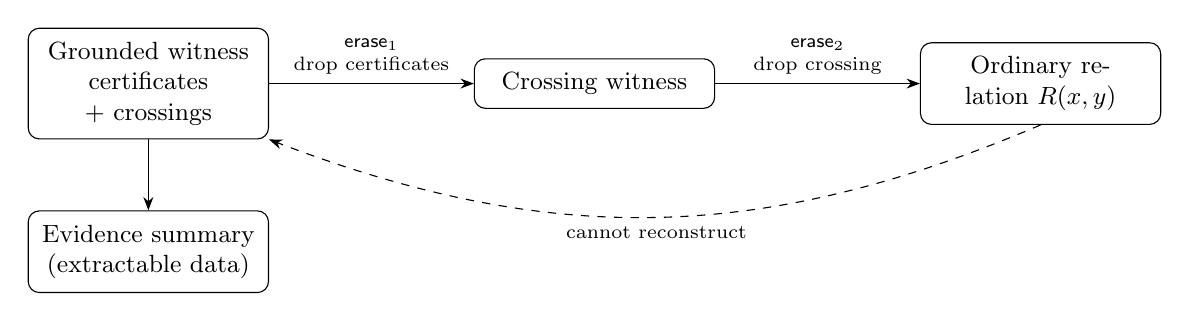
\begin{tikzpicture}[node distance=9mm and 26mm, box/.style={draw,rounded corners,align=center,inner sep=5pt,font=\small,text width=2.7cm}, lab/.style={align=center,font=\scriptsize}, >=Stealth]
\node[box] (G) {Grounded witness\\ certificates $+$ crossings};
\node[box,right=of G] (C) {Crossing witness};
\node[box,right=of C] (R) {Ordinary relation $R(x,y)$};
\node[box,below=of G] (S) {Evidence summary (extractable data)};
\draw[->] (G) -- node[above,lab]{$\erase_1$\\ drop certificates} (C);
\draw[->] (C) -- node[above,lab]{$\erase_2$\\ drop crossing} (R);
\draw[->] (G) -- (S);
\draw[->,dashed,bend left=22] (R.south) to node[below,lab]{cannot reconstruct} (G.south east);
\end{tikzpicture}
\caption{Two-stage erasure. The dashed arrow marks what erasure loses irreversibly (\cref{thm:nonreflect,thm:multiplicity}). The evidence summary is a separate, lossy projection that keeps extractable identifiers.}
\label{fig:erasure}
\end{figure}

\paragraph{First erasure.}
$\erase_1 : \GTrans_c(s,t) \to \Cross_c(s,t)$ maps $\mathsf{step}(r,\kappa)$ to the crossing $\mathsf{step}(r)$ justified by the grounding equations contained in $\kappa$, and is the identity on $\mathsf{id}$ and $\cdot$ (\coq{rpath_forget}). It forgets the lineage graph, coverage and gaps, custodian, authority evidence, maintenance evidence, and the identity of the certificate; it keeps the directed path and the seam elements crossed.

\paragraph{Second erasure.}
$\erase_2 : \Cross_c(s,t) \to R_c(s,t)$ maps a crossing path to agreement $\val(s) = \val(t)$ (\cref{thm:soundness}). It forgets which crossing was used, whether there was more than one, and the internal structure of the transition. The composite $\erase = \erase_2 \circ \erase_1$ is ordinary substitutability. Both stages preserve identity and composition.

\begin{table}[t]
\centering\small
\caption{Grounded versus ordinary rewriting.}\label{tab:compare}
\begin{tabularx}{\textwidth}{@{}lYY@{}}
\toprule
 & Ordinary rewriting & Grounded transport \\
\midrule
Judgement & $R(x,y) : \Prop$ & $\GTrans_c(x,y) : \Type$ \\
Inhabitants & indistinguishable proofs & distinguishable witnesses \\
Seam, lineage, coverage & not retained & retained as data \\
Contexts & $\Proper$: preserves the relation & crossing-proper / certificate-proper: map witnesses \\
Failure & absence of proof & located obstruction, or open obligation \\
Relation to the other & --- & erases to it; not conversely \\
\bottomrule
\end{tabularx}
\end{table}

\subsection{Erasure soundness}
\begin{thm}[Erasure soundness]\label{thm:soundness}
If $w : \GTrans_c(s,t)$ then $\val(s) = \val(t)$. \emph{(Coq: \coq{erase_sound}, \coq{rpath_sound}; generically \coq{erasure_sound}.)}
\end{thm}
\begin{proof}
By induction on $w$, through $\erase_1$. If $w = \mathsf{id}_s$, reflexivity. If $w = \mathsf{step}(r,\kappa)$, the construction certificate in $\kappa$ contains the grounding equations at $r$, so
\[
\val(\mathsf{inl}\,\back(r)) = \Phi_A(\back(r)) = \Phi_\Sigma(r) = \Phi_B(\fwd(r)) = \val(\mathsf{inr}\,\fwd(r)).
\]
If $w = v \cdot v'$, combine the hypotheses for $v$ and $v'$ by transitivity.
\end{proof}
For a generic transport structure $G$ for $R$ write $\erased_G(x,y) :\equiv \|\GTrans_G(x,y)\|$.
\begin{prop}[Erased preorder]\label{prop:preorder}
$\erased_G$ is reflexive and transitive, and contained in $R$. \emph{(Coq: \coq{erased_PreOrder}, \coq{erasure_sound}.)}
\end{prop}
\begin{proof}
Reflexivity from $\mathsf{id}$, transitivity from composition, containment from the soundness map of $G$.
\end{proof}
Since composition is associative only up to $\weq$ (\cref{thm:algebra}) but $\erased_G$ records only inhabitation, the erased relation satisfies the ordinary preorder laws with no qualification.

\subsection{Sound refinement, not universal reconstruction}
Two formulations must be distinguished. If the relation is \emph{defined} by the existence of a grounded witness, $R_G(x,y) :\Longleftrightarrow \exists w : \GTrans_G(x,y)$, then erasure characterises $R_G$ exactly, by definition. If instead $R$ is independently given, the general theorem is only the soundness map $\GTrans_G(x,y) \to R(x,y)$. A converse requires a completeness (representability) hypothesis.
\begin{prop}[Exact recovery under completeness]\label{prop:complete}
Call $G$ \emph{complete} if $R(x,y) \Rightarrow \erased_G(x,y)$ for all $x,y$. Then $R$ and $\erased_G$ coincide. Completeness holds for the trivial structure whose witnesses are the proofs $R(x,y)$ themselves (for a preorder $R$), and is refuted by any $R$-related pair without a witness. \emph{(Coq: \coq{erasure_exact_of_complete}, \coq{preorder_complete}, \coq{not_complete_of_gap}.)}
\end{prop}
It fails in exactly the cases of interest (\cref{thm:nonreflect}). We therefore call the generic result a \emph{sound refinement}, not an equivalence with all ordinary rewriting, and we do not say that grounded transport ``recovers'' all ordinary rewriting.

\subsection{Non-reflection}
\begin{thm}[Erasure does not reflect grounding]\label{thm:nonreflect}
There exist a transport problem $c$ and states $s,t$ with $\val(s) = \val(t)$ and $\neg\,\erased_{\GTrans_c}(s,t)$. \emph{(Coq: \coq{erasure_not_reflecting}, \coq{copied_ungrounded_agreement}.)}
\end{thm}
\begin{proof}
Let $c_{\mathrm{dw}}$ be the dual-write problem of \cref{sec:example}: $\Sigma = A = B = \{r_{\mathrm{ok}}, r_*\}$, $\back = \fwd = \mathrm{id}$, $\Phi_A = \Phi_B \equiv 1$, $\Phi_\Sigma(r_{\mathrm{ok}}) = 1$, $\Phi_\Sigma(r_*) = 0$, with maintenance and authority evidence trivially inhabited by a one-point type, constant observation maps (so both coordinates are admissible), and the declared lineage record $\ell$ with nodes $0$ (raw status), $1 = d_A$ with parent $0$, $2 = d_B$ with parent $1$, and ground node $3 = g$ with parent $1$. Thus the ground is derived from $d_A$.

\emph{Step 1: $\mathsf{Cert}(c_{\mathrm{dw}}) = \emptyset$.} Suppose $\kappa \in \mathsf{Cert}(c_{\mathrm{dw}})$. Its construction certificate contains a lineage certificate $\lambda$ with graph $\ell$ and a proof of L1 for $\ell$, so $d_A = 1 \notin \anc_\ell(3)$. But $1 \in \mathsf{parents}_\ell(3)$, so $1 \in \anc_\ell(3)$, a contradiction. (Independently, the grounding equation at $r_*$ would require $\Phi_A(r_*) = 1 = 0 = \Phi_\Sigma(r_*)$.)

\emph{Step 2: every $w \in \GTrans_{c_{\mathrm{dw}}}(s,t)$ has $s = t$.} By induction on $w$: identity is trivial; a $\mathsf{step}$ would contain a certified transport, impossible by Step 1; and if $s = s'$ and $s' = t$ then $s = t$.

\emph{Step 3.} Take $s = \mathsf{inl}\,r_*$ and $t = \mathsf{inr}\,r_*$. Then $\val(s) = \Phi_A(r_*) = 1 = \Phi_B(r_*) = \val(t)$, but $s \neq t$ (different summands). By Step 2 there is no witness, so $\erased(s,t)$ fails.
\end{proof}
The same fact is a generic \emph{ungrounded agreement}: extensional agreement without a transport witness, whose existence refutes completeness and hence exact recovery.

\subsection{Same endpoints, different warrants}\label{sec:multiplicity}
Non-reflection shows that erasure has no inverse. A stronger result gives two \emph{positive} witnesses for the same endpoints whose evidential difference is observable before erasure. Witnesses for different problems have different indexed types, so we package the problem with the witness.
\begin{defi}[Packed warrants]\label{def:packed}
Fix an endpoint type $E$ and, for each problem $c$, an interpretation $\mathsf{emb}_c : S_c \to E$. Then
\[
\mathsf{PackedWarrant}(x,y) \;:\equiv\; \sum_{c}\ \sum_{s,t : S_c} \bigl(\mathsf{emb}_c(s) = x\bigr) \times \bigl(\mathsf{emb}_c(t) = y\bigr) \times \GTrans_c(s,t),
\]
and $\mathsf{ErasedAt}(x,y) :\equiv \exists c, s, t.\ \mathsf{emb}_c(s) = x \wedge \mathsf{emb}_c(t) = y \wedge \erased_{\GTrans_c}(s,t)$. Erasure of a packed warrant lands in $\mathsf{ErasedAt}(x,y)$. The \emph{extractable summary} $\mathsf{summary}(w)$ of a witness is the list, over its crossings, of: exhibition record identifier, custodian, lineage ground node, coverage interval, number of declared lineage dispositions, and the maintenance and authority summaries supplied by the application's evidence-summary interface (\cref{sec:mechanisation}).
\end{defi}
This places warrants from problems with \emph{different} declared lineage into one endpoint-indexed collection, without pretending their lineage records coincide. (Coq: \coq{PackedWarrant}, \coq{erase_packed}, \coq{warrant_summary}.)

\begin{thm}[Same endpoints, different warrants]\label{thm:multiplicity}
There exist $w_1, w_2 \in \mathsf{PackedWarrant}(x,y)$ for the same endpoints such that both erase into $\mathsf{ErasedAt}(x,y)$, while $\mathsf{summary}(w_1) \neq \mathsf{summary}(w_2)$, and hence $w_1 \neq w_2$. Within a single problem, two witnesses in $\GTrans_c(s,t)$ have different summaries. \emph{(Coq: \coq{packed_warrants_same_endpoints}, \coq{same_endpoints_different_warrants}, \coq{packed_distinguishable}.)}
\end{thm}
\begin{proof}
Let $E = \bool$, with $\mathsf{emb}_c$ sending $A$-side states to $0$ and $B$-side states to $1$. For a list $d$ of lineage dispositions let $c_d$ be the problem with $A = B = \{\ast\}$, $\Sigma = \{0,1\}$ (two seam elements), all valuations constantly $1$, trivial observation maps, maintenance evidence a point, authority evidence a record $(\text{authority identifier})$, and declared lineage the record $\ell_d$: raw nodes $0,1,2$; $d_A = 3$ with parent $0$; $d_B = 4$ with parent $1$; ground $5$ with parent $2$; $\{2\}$ the claim-relevant inputs; dispositions $d$. The graph $\ell_d$ is well-formed and satisfies L1--L3: the ancestors of $3$, $4$, $5$ are $\{0\}$, $\{1\}$, $\{2\}$ respectively, so the ground descends from neither coordinate, there are no shared non-raw ancestors, and $2$ is a claim-relevant raw input among the ground-only ancestors. Hence for every choice of record identifier $\rho$, custodian $\varsigma$, authority $\alpha$ and coverage $\gamma$ we obtain a certified transport $\kappa(d,\rho,\varsigma,\alpha,\gamma) \in \mathsf{Cert}(c_d)$: admissibility from the constant factor, the grounding equations hold as all valuations are $1$, and the exhibition certificate is $(\rho, \iota, \text{process}, \mathrm{Ret} = \bool, \mathsf{retain} = \Phi_\Sigma, \mathsf{eval} = \mathrm{id}, \gamma, \varsigma)$ with $\iota$ injective.

Let $d_0 = [\,]$ and $d_1 = [(9,\mathsf{Justified})]$, and put
\begin{align*}
w_1 &= \mathsf{step}(0, \kappa(d_0, 1, 7, 11, (0,1))) && \in \GTrans_{c_{d_0}}(\mathsf{inl}\,\ast, \mathsf{inr}\,\ast),\\
w_2 &= \mathsf{step}(1, \kappa(d_0, 2, 8, 12, (0,5))) && \in \GTrans_{c_{d_0}}(\mathsf{inl}\,\ast, \mathsf{inr}\,\ast),\\
w_3 &= \mathsf{step}(0, \kappa(d_1, 1, 7, 11, (0,1))) && \in \GTrans_{c_{d_1}}(\mathsf{inl}\,\ast, \mathsf{inr}\,\ast).
\end{align*}
All have endpoints $(0,1)$ under $\mathsf{emb}$, so pack to elements of $\mathsf{PackedWarrant}(0,1)$, and all erase into $\mathsf{ErasedAt}(0,1)$ by $\erase$. Their summaries list, for $w_1,w_2,w_3$ respectively: record identifiers $1,2,1$; custodians $7,8,7$; coverage intervals $(0,1),(0,5),(0,1)$; authorities $11,12,11$; and $0,0,1$ declared lineage dispositions (all with ground node $5$). These differ pairwise: $w_1,w_2$ in record, custodian, coverage and authority; $w_1,w_3$ in the number of lineage dispositions. Since equal witnesses have equal summaries, $w_i \neq w_j$ for $i \neq j$.
\end{proof}
We do not assert equality of the two erased \emph{proofs}: $\mathsf{ErasedAt}$ is a proposition, so equality of its proofs would require proof irrelevance and would be uninformative. The content is that erasure sends both witnesses into a single proposition that records nothing about which was used, while the summary separates them. The witnesses differ in seam element, exhibition record, custodian, coverage interval, authority, and, across problems, in the declared lineage. This is the most direct proof that ordinary rewriting forgets evidential structure.

\subsection{Observational agreement is not a warrant}\label{sec:obstruction}
Non-reflection concerns the relation induced by transport. A related question is whether an \emph{observational} equivalence can license substitution for a predicate that depends on lineage. Let $M : X \to O$ be an observation map, $x \sim_M y :\Leftrightarrow M(x) = M(y)$, and $P : X \to V$ a predicate. Recall that $P$ \emph{factors through} $M$ iff $P = h \circ M$ for some $h$, which holds iff $P$ is constant on the fibres of $M$; this is the standard factorisation criterion \cite{cousot1977}.
\begin{prop}[Observational agreement cannot license lineage-sensitive substitution]\label{prop:obsobstruction}
Suppose $x \sim_M y$ and $P(x) \neq P(y)$. Then
(a) $P$ does not factor through $M$, and $P$ is not proper for $(\sim_M, =)$;
(b) if $G$ is a transport structure for the relation $R_P(a,b) :\equiv P(a) = P(b)$, then $\GTrans_G(x,y)$ is empty.
Consequently no transport structure sound for $R_P$ is complete for $\sim_M$. \emph{(Coq: \coq{fibre_obstruction}, \coq{not_proper_of_distinguished}, \coq{observational_not_grounded}, \coq{obs_equiv_not_transport}.)}
\end{prop}
\begin{proof}
(a) If $P = h \circ M$ then $P(x) = h(M(x)) = h(M(y)) = P(y)$, contradicting $P(x) \neq P(y)$; and properness would give $P(x) = P(y)$ from $x \sim_M y$. (b) A witness $w \in \GTrans_G(x,y)$ would give $R_P(x,y)$ by soundness, that is $P(x) = P(y)$. The last claim follows since completeness for $\sim_M$ would give $\GTrans_G(x,y)$ from $x \sim_M y$.
\end{proof}
In the dual-write example take $M$ to be the copied coordinate value (constant $1$) and $P(\mathsf{inl}\,r) = \Phi_\Sigma(r)$, the exhibited trace status: $P(\mathsf{inl}\,r_{\mathrm{ok}}) = 1 \neq 0 = P(\mathsf{inl}\,r_*)$, although $M$ identifies them. So the trace status is not determined by the copied value (\coq{trace_not_determined_by_copied_value}). The direction from factorisation to fibre-constancy and its relational converse are constructive; the finite converse needs a complete enumeration and decidable equality; the unrestricted functional converse needs classical choice and is isolated (\cref{sec:mechanisation}).

\section{The grounded-seam instance}\label{sec:seams}

This section connects the calculus to an earlier grounded-seam development \cite{moore2026} without requiring the reader to consult it: we restate the definitions and the theorem being recovered.

\subsection{Grounding equations}
A span $A \xleftarrow{\back} \Sigma \xrightarrow{\fwd} B$ carries Boolean valuations $\Phi_A$, $\Phi_B$ and a seam valuation $\Phi_\Sigma$. The \emph{grounding equations} require both coordinate valuations to agree with the independently exhibited seam valuation:
\[
\mathsf{GE}:\qquad \Phi_A(\back(r)) = \Phi_\Sigma(r) \quad\text{and}\quad \Phi_B(\fwd(r)) = \Phi_\Sigma(r) \qquad (r \in \Sigma).
\]
\emph{Extensional seam agreement} is only pairwise: $\mathsf{EA}:\ \Phi_A(\back(r)) = \Phi_B(\fwd(r))$ for all $r$. A crossing witness $\mathsf{step}(r)$ (\cref{def:gtrans}) is exactly a crossing at which $\mathsf{GE}$ holds; the compatibility layer takes states to be $A + B$ and crossing witnesses as in \cref{def:gtrans}. An earlier reconstruction of this instance used only $\mathsf{EA}$ as the seam condition; it collapsed exactly the distinction this paper concerns, and survives in the development only as a clearly labelled weaker layer.

\subsection{Grounding erases to pairwise agreement}
\begin{prop}[Grounding erases]\label{prop:groundingerases}
$\mathsf{GE} \Longrightarrow \mathsf{EA}$, that is, $\Phi_A \circ \back = \Phi_B \circ \fwd$. \emph{(Coq: \coq{original_grounding_erases_to_extensional}.)}
\end{prop}
\begin{proof}
For $r \in \Sigma$, $\mathsf{GE}$ supplies a crossing witness $\mathsf{step}(r) \in \Cross(\mathsf{inl}\,\back(r), \mathsf{inr}\,\fwd(r))$; erasure soundness (\cref{thm:soundness}, at the crossing level) gives $\Phi_A(\back(r)) = \Phi_B(\fwd(r))$. Directly: $\Phi_A(\back(r)) = \Phi_\Sigma(r) = \Phi_B(\fwd(r))$.
\end{proof}

\subsection{The converse fails}
\begin{prop}[Pairwise agreement does not imply grounding]\label{prop:pairwise}
There exist a span and valuations satisfying $\mathsf{EA}$ but not $\mathsf{GE}$. \emph{(Coq: \coq{pairwise_agreement_not_grounding}, from \coq{copied_extensionally_coherent} and \coq{copied_not_grounded}.)}
\end{prop}
\begin{proof}
Take the dual-write span of \cref{sec:example}: $\Sigma = A = B = \{r_{\mathrm{ok}}, r_*\}$, $\back = \fwd = \mathrm{id}$, $\Phi_A = \Phi_B \equiv 1$, $\Phi_\Sigma(r_{\mathrm{ok}}) = 1$, $\Phi_\Sigma(r_*) = 0$. For every $r$, $\Phi_A(\back(r)) = 1 = \Phi_B(\fwd(r))$, so $\mathsf{EA}$ holds. But $\mathsf{GE}$ at $r_*$ would give $\Phi_A(\back(r_*)) = \Phi_\Sigma(r_*)$, that is, $1 = 0$. So $\mathsf{GE}$ fails. (If $\mathsf{EA}$ implied $\mathsf{GE}$ for all spans, it would in particular for this one.)
\end{proof}
The generic reading is \cref{thm:nonreflect}: the legacy counterexample embeds as ungrounded agreement in the generic calculus, and, conversely, \coq{copied_not_grounded} is recovered from the generic obstruction (\coq{original_copied_counterexample_embeds}, \coq{copied_not_grounded_from_generic}).

\subsection{Recovering the original theorem}
The earlier work proves the following \emph{seam transport theorem}: let $M_A : A \to O_A$, $h : O_A \to \bool$, and suppose $\Phi_A = h \circ M_A$.
\begin{thm}[Seam transport \cite{moore2026}]\label{thm:seamtransport}
If $\mathsf{GE}$ holds then for every $r \in \Sigma$, $\ \Phi_B(\fwd(r)) = h(M_A(\back(r)))$. \emph{(Coq legacy statement: \coq{seam_transport}; recovered as \coq{original_seam_transport_from_generic}.)}
\end{thm}
The compatibility layer proves that the definitions of the earlier work instantiate the generic calculus and derives \cref{thm:seamtransport} \emph{with the statement unchanged}, in two steps that make its logical strength explicit.
\begin{prop}[Extensional factor transport]\label{prop:extfactor}
If $\mathsf{EA}$ holds and $\Phi_A = h \circ M_A$ then $\Phi_B(\fwd(r)) = h(M_A(\back(r)))$ for every $r$. \emph{(Coq: \coq{extensional_factor_transport}.)}
\end{prop}
\begin{proof}
$\Phi_B(\fwd(r)) = \Phi_A(\back(r)) = h(M_A(\back(r)))$, by $\mathsf{EA}$ and the factorisation.
\end{proof}
\begin{cor}[Grounded factor transport]\label{cor:groundedfactor}
$\mathsf{GE}$ and $\Phi_A = h \circ M_A$ imply $\Phi_B(\fwd(r)) = h(M_A(\back(r)))$. \emph{(Coq: \coq{grounded_factor_transport}.)}
\end{cor}
\begin{proof}
By \cref{prop:groundingerases}, $\mathsf{GE} \Rightarrow \mathsf{EA}$; apply \cref{prop:extfactor}.
\end{proof}
The logical strength is worth stating plainly, and it is a positive result, not a concession:
\begin{quote}
\emph{The endpoint equality requires only pairwise extensional agreement and the supplied factorisation. The grounded witness does not change that equality; it records why applying the equality is warranted.}
\end{quote}
The conclusion of \cref{thm:seamtransport} can remain true after the warrant supporting it has failed (\coq{extensional_conclusion_survives_ungrounded}): on the dual-write span the endpoint equation holds at every $r$ with the constant factor, while $\mathsf{GE}$ fails. That is precisely what non-reflection expresses. A reader who observes that the earlier theorem has stronger premises than its conclusion needs is correct, and the observation is part of the contribution.

\subsection{Legacy preservation}
The earlier supplement is retained byte-for-byte and built as a separate library; its authoritative checksums match; its own build-and-check procedure completes; and the new development imports it through a compatibility layer. The original theorem is recovered, not silently redefined. The checksum table belongs to the artefact documentation, not to this paper.

\section{Dynamic preservation and failure}\label{sec:dynamic}

\Cref{sec:seams} concerns one stage. This section asks what survives when the system evolves, and separates four notions that are easily conflated: structural naturality, valuation naturality, preservation of grounding, and coverage.

\subsection{Structural naturality}
A \emph{seam evolution} $U$ from stage $t$ to stage $u$ consists of maps $U^\Sigma : \Sigma_t \to \Sigma_u$, $U^A : A_t \to A_u$, $U^B : B_t \to B_u$ such that the squares commute:
\[
\back_u \circ U^\Sigma = U^A \circ \back_t, \qquad \fwd_u \circ U^\Sigma = U^B \circ \fwd_t.
\]
Evolutions have identity and composition (componentwise), and commutation composes: the composite of two evolutions commutes. Its state map $\mathsf{inl}\,a \mapsto \mathsf{inl}(U^A a)$, $\mathsf{inr}\,b \mapsto \mathsf{inr}(U^B b)$ agrees pointwise with the composite of the state maps of the steps, so the composite evolution and $\mathsf{gp\_comp}$ of the steps act identically (\coq{evo_state_id}, \coq{evo_state_compose}, \coq{evolution_compose_via_gp_comp}). The squares say nothing about valuations.

\subsection{Valuational preservation}\label{sec:valuational}
If the value spaces carry a transport $U^V : \bool \to \bool$, one may additionally require \emph{valuation naturality}, of all three valuations:
\[
\Phi_{A,u} \circ U^A = U^V \circ \Phi_{A,t}, \quad
\Phi_{B,u} \circ U^B = U^V \circ \Phi_{B,t}, \quad
\Phi_{\Sigma,u} \circ U^\Sigma = U^V \circ \Phi_{\Sigma,t}.
\]
Values need not stay unchanged: requiring $U^V = \mathrm{id}$ would turn a dynamic predicate into a temporal invariant. Write $\mathsf{GE}_t(r)$ for the grounding equations at $r \in \Sigma_t$ and define
\[
\mathsf{PreservesGroundingOnImage}(U) \;:\Longleftrightarrow\; \forall r \in \Sigma_t.\ \mathsf{GE}_t(r) \Rightarrow \mathsf{GE}_u(U^\Sigma(r)).
\]
This property concerns only seam elements \emph{of the form} $U^\Sigma(r)$, and says nothing about target elements outside the image. (In the development it is called \coq{PreservesGroundingOnImage}.)

\begin{thm}[Naturality preserves grounding on the image]\label{thm:preserve}
If the structural squares commute and all three valuations are natural with respect to some $U^V$, then $\mathsf{PreservesGroundingOnImage}(U)$. In particular if $\mathsf{GE}$ holds at every element of $\Sigma_t$ then $\mathsf{GE}_u$ holds at every transported element. \emph{(Coq: \coq{natural_valuations_preserve_grounding_on_image}, \coq{grounding_at_transported_elements}.)}
\end{thm}
\begin{proof}
Let $\mathsf{GE}_t(r)$ hold. Then
\begin{align*}
\Phi_{A,u}(\back_u(U^\Sigma r)) &= \Phi_{A,u}(U^A(\back_t r)) && \text{(back square)}\\
&= U^V(\Phi_{A,t}(\back_t r)) && \text{(naturality of $\Phi_A$)}\\
&= U^V(\Phi_{\Sigma,t}(r)) && \text{($\mathsf{GE}_t(r)$)}\\
&= \Phi_{\Sigma,u}(U^\Sigma r) && \text{(naturality of $\Phi_\Sigma$)},
\end{align*}
and symmetrically for $B$ with the fwd square.
\end{proof}
Naturality is preserved by identity and composition, with $U^V$ composing (\coq{natural_id}, \coq{natural_compose}).

\begin{thm}[Global preservation under coverage]\label{thm:coverage}
If $U^\Sigma$ is surjective, $U$ preserves grounding on the image, and $\mathsf{GE}_t(r)$ holds for all $r \in \Sigma_t$, then $\mathsf{GE}_u(r')$ holds for all $r' \in \Sigma_u$. \emph{(Coq: \coq{surjective_evolution_preserves_all_grounding}.)}
\end{thm}
\begin{proof}
Let $r' \in \Sigma_u$. By surjectivity $r' = U^\Sigma(r)$ for some $r$; apply preservation to $\mathsf{GE}_t(r)$.
\end{proof}
Without surjectivity, new target elements require new grounding evidence: there is a model in which preservation on the image holds and every stage-$t$ element is grounded, yet a stage-$u$ element outside the image is not (\coq{preservation_without_coverage}). Preservation of grounding therefore separates \emph{continuation} from \emph{coverage}, and matches the reading that a new process requires a new certificate (\cref{fig:dynamic}).

\begin{figure}[t]
\centering
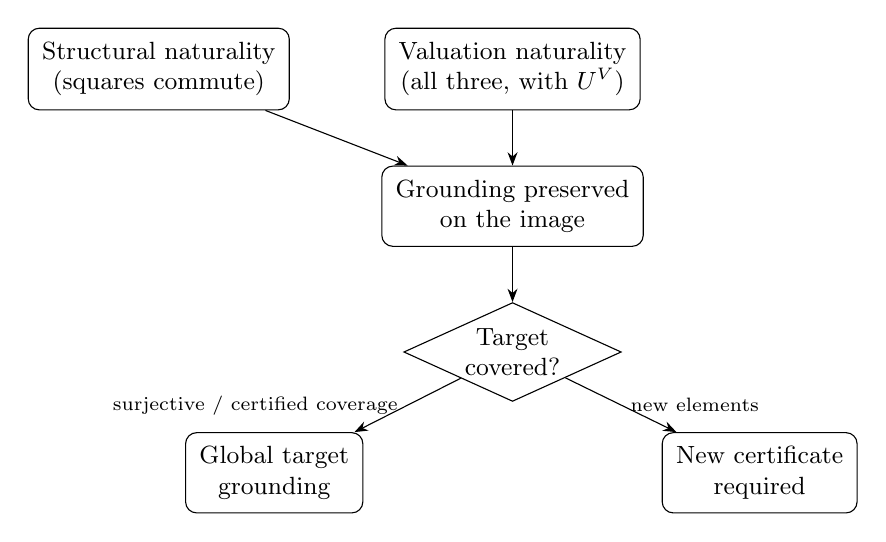
\begin{tikzpicture}[node distance=7mm and 12mm, box/.style={draw,rounded corners,align=center,inner sep=5pt,font=\small}, dia/.style={draw,diamond,aspect=2.2,align=center,inner sep=1pt,font=\small}, >=Stealth]
\node[box] (S) {Structural naturality\\ (squares commute)};
\node[box,right=of S] (V) {Valuation naturality\\ (all three, with $U^V$)};
\node[box,below=of V] (G) {Grounding preserved\\ on the image};
\node[dia,below=of G] (C) {Target\\ covered?};
\node[box,below left=of C] (A) {Global target\\ grounding};
\node[box,below right=of C] (N) {New certificate\\ required};
\draw[->] (S) -- (G);
\draw[->] (V) -- (G);
\draw[->] (G) -- (C);
\draw[->] (C) -- node[left,font=\scriptsize]{surjective / certified coverage} (A);
\draw[->] (C) -- node[right,font=\scriptsize]{new elements} (N);
\end{tikzpicture}
\caption{Structural and valuational preservation. Structure alone does not give preservation of grounding; preservation alone does not give coverage.}
\label{fig:dynamic}
\end{figure}

\subsection{Evolutions as contexts, at both levels}
A seam evolution $U$ that preserves grounding on the image is a \emph{crossing-proper} context between the crossing structures at the two stages (\coq{evolution_crossing_proper}, built on \coq{original_grounding_preserving_evolution_is_grounded_proper}), acting on states by $\mathsf{inl}\,a \mapsto \mathsf{inl}(U^A a)$, $\mathsf{inr}\,b \mapsto \mathsf{inr}(U^B b)$ and on crossed seam elements by $U^\Sigma$. On a crossing at $r$ it produces the crossing at $U^\Sigma(r)$, its grounding equations supplied by preservation, with endpoints transported along the two squares. Identity and composition of witnesses are respected, so \cref{thm:twolevels} applies and composite evolutions are crossing-proper (\coq{evolution_compose_grounded_proper}). The hypothesis is exposed in the name because the witness map must send a grounded crossing at $r$ to a grounded crossing at its image.

Crossing-proper preservation carries no certificates. For an evolution to be \emph{certificate-proper} it must come with an evidence lift (\cref{def:pm}): a way to turn certified transports at stage $t$ into certified transports at stage $u$. Two models with the same structure show that this is a genuine additional requirement.
\begin{thm}[Certificate reissue, and its impossibility]\label{thm:reissue}
Consider the two-stage model of \cref{thm:dynfail} with the problems $c_0$ and $c_1$ at stages $0$ and $1$ (trivial maintenance, authority and observation evidence, and the independent lineage record of \cref{sec:multiplicity}).
(a) If the seam valuation is $1$ at both stages, there is a problem morphism $c_0 \to c_1$ whose lift \emph{reissues} a certificate at stage $1$; hence its state map is certificate-proper.
(b) If, as in \cref{thm:dynfail}, $\Phi_{\Sigma,1}(\ast) = 0$ while $\Phi_{\Sigma,0}(\ast) = 1$, there is \emph{no} problem morphism $c_0 \to c_1$.
\emph{(Coq: \coq{reissue_certificate_proper}, \coq{no_evidence_lift_when_grounding_lost}.)}
\end{thm}
\begin{proof}
(a) All components are the unique maps into or out of $\{\ast\}$, so the squares commute and grounding is preserved (both sides are $1 = 1$). For the lift, note that a certified transport for $c_1$ exists: the exhibition certificate uses $\mathrm{Ret} = \bool$ with $\mathsf{retain} = \Phi_{\Sigma,1}$ and $\mathsf{eval} = \mathrm{id}$, the lineage certificate is that of the independent record, and the grounding equations at stage $1$ read $1 = 1$. Let the lift send every certified transport of $c_0$ to this one. \cref{thm:lifting} makes the state map certificate-proper.
(b) A certified transport for $c_0$ exists: the same construction at stage $0$, where the equations read $1 = 1$. Any evidence lift would send it to a certified transport for $c_1$, whose construction certificate contains the grounding equation $\Phi_{A,1}(\back\ast) = \Phi_{\Sigma,1}(\ast)$, that is $1 = 0$, a contradiction.
\end{proof}
In these two models, loss of grounding prevents any evidence lift, while the grounded target permits the particular reissue lift supplied in (a). This is not a general equivalence: preservation of grounding alone need not provide exhibition, lineage, maintenance or authority evidence at the target. In (b) the evolution does not preserve grounding on the image (\cref{thm:dynfail}), so the crossing-level instance above is unavailable as well; and where the crossing-level instance exists, as in (a), the certificate-level instance still needs an evidence lift, which we supply only by reissuing. A general theory of maintaining exhibition records and lineage across evolutions, rather than reissuing them, is left open (\cref{sec:limitations}).

\subsection{The dynamic separation theorem}
\begin{thm}[Extensional persistence without grounded preservation]\label{thm:dynfail}
There is a seam evolution such that
(1) the structural squares commute;
(2) extensional agreement holds at both stages;
(3) ordinary factor transport remains valid at the later stage;
(4) grounding holds at the earlier stage;
(5) grounding fails at a transported seam element.
\emph{(Coq: \coq{dynamic_failure_visible}, \coq{ordinary_rewriting_still_succeeds}, \coq{structural_naturality_not_preservation}.)}
\end{thm}
\begin{proof}
Take two stages $0,1$ and $\Sigma_t = A_t = B_t = \{\ast\}$ at each, with all projections the unique map. Let $\Phi_{A,t} = \Phi_{B,t} \equiv 1$ at both stages, $\Phi_{\Sigma,0}(\ast) = 1$ and $\Phi_{\Sigma,1}(\ast) = 0$. Let $U$ be the unique evolution (all components the unique maps).
(1) All maps into $\{\ast\}$ are equal, so both squares commute.
(2) At each stage $\Phi_A(\back(\ast)) = 1 = \Phi_B(\fwd(\ast))$.
(3) With $M_A$ constant and $h \equiv 1$ we have $\Phi_A = h \circ M_A$, and $\Phi_B(\fwd(\ast)) = 1 = h(M_A(\back(\ast)))$ at stage $1$; this is \cref{prop:extfactor} at stage $1$.
(4) At stage $0$: $\Phi_{A,0}(\back \ast) = 1 = \Phi_{\Sigma,0}(\ast)$ and likewise for $B$.
(5) The unique transported element is $U^\Sigma(\ast) = \ast \in \Sigma_1$, and $\Phi_{A,1}(\back \ast) = 1 \neq 0 = \Phi_{\Sigma,1}(\ast)$, so $\mathsf{GE}_1(\ast)$ fails.
\end{proof}
Consequently $\mathsf{PreservesGroundingOnImage}(U)$ fails, although every squares-commute and agreement condition holds. This is the formal maintenance result: the warrant was valid at issuance, the system evolved, and the coordinates continue to agree while the independently evolved ground no longer agrees with them.

\subsection{Interpretation}
Structural naturality preserves the relationship between carriers and coordinates. It does not automatically preserve the relationship between those coordinates and their independently grounded valuation, nor the certificates attesting to it. Maintenance evidence is therefore distinct from extensional preservation: a migration whose squares commute can be structurally faithful and evidentially stale. We call the located counterexample to such preservation a \emph{maintenance obstruction} (\cref{sec:assessment}).

\section{Evidence-bearing assessment}\label{sec:assessment}

\subsection{Component states}
Each of four obligations of a problem $c$ is assessed separately. For an obligation with evidence type $E$ and located-failure type $F$, a \emph{component verdict} is one of
\[
\mathsf{Discharged}(e),\quad e \in E; \qquad \mathsf{Failed}(f),\quad f \in F; \qquad \mathsf{Unresolved}(o),
\]
where $o$ names the missing evidence or decision (a not-yet-assessed obligation, a missing lineage record, a declared coverage gap, an incomplete search, or an undeclared policy). The four obligations are \emph{observation} ($E = \Adm(M_A,\Phi_A) \wedge \Adm(M_B,\Phi_B)$), \emph{construction} ($E = \mathsf{Con}(c)$), \emph{maintenance} ($E = \mathrm{Mnt}$) and \emph{institution} ($E = \mathrm{Aut}$).

\subsection{Located evidence}
A failure names the defect, and where possible carries data locating it, rather than being merely a proof of a negated proposition (\cref{tab:failures}). Each carries a proof that it refutes the corresponding evidence, so it is a counter-argument.
\begin{table}[t]
\centering\small
\caption{Located failures, the evidence each refutes, and what each carries. \emph{Data} survives extraction; \emph{proof} does not (only the constructor tag remains).}\label{tab:failures}
\begin{tabularx}{\textwidth}{@{}llYY@{}}
\toprule
Obligation & Failure & Conjunct refuted & Carries \\
\midrule
Observation & fibre witness ($A$ or $B$) & $\Adm(M,\Phi)$ & data: states $s_1,s_2$; proof: $M s_1 = M s_2$, $\Phi s_1 \neq \Phi s_2$ \\
Construction & empty seam & $\mathsf{Inh}(\Sigma)$ & --- \\
 & grounding failure & $\mathsf{GE}$ & data: seam element $r$; proof: which equation fails \\
 & exhibition defeated & $\mathsf{Inh}(\mathsf{Exh}(c))$ & --- \\
 & coordinate-ground identity & L1 & proof: the ground node equals a coordinate node (tag only after extraction) \\
 & lineage descent & L1 & proof: an ancestor derivation from a coordinate to the ground (tag only after extraction) \\
 & undisclosed shared ancestor & L2 & data: the node $n$; proof: it is a shared, non-raw, undispositioned ancestor \\
 & no independent source & L3 & --- \\
 & malformed record & well-formedness & proof of the violation; the checker of \cref{sec:lineage} additionally reports which condition \\
Maintenance & lost grounding, or no evolution & $\mathsf{Inh}(\mathrm{Mnt})$ & data: for every evolution, a seam element where grounding is lost \\
Institution & application-defined & $\mathsf{Inh}(\mathrm{Aut})$ & application-defined \\
\bottomrule
\end{tabularx}
\end{table}
The maintenance failure of \cref{thm:dynfail} is the typical case: for the unique evolution the seam element $\ast$ is grounded at stage $0$ and its image is not grounded at stage $1$.

\subsection{Report and verdict}
We keep two things apart: the complete component \emph{report}, and its aggregate \emph{verdict}.
\begin{defi}[Assembly]\label{def:assembly}
Given component verdicts $v_1,\dots,v_4$ (in the order observation, construction, maintenance, institution), let $\mathsf{failures}$ be the list of located failures among them, in that order; $\mathsf{opens}$ the list of unresolved obligations; and $\mathsf{discharged}$ the list of discharged ones. The \emph{report} is the triple $(\mathsf{failures},\mathsf{opens},\mathsf{discharged})$. The \emph{assessment} $\mathsf{assemble}(v_1,\dots,v_4)$ is
\[
\begin{cases}
\Refu(\mathsf{failures}) & \text{if } \mathsf{failures} \neq [\,],\\
\Cert(\kappa) & \text{if all four are discharged, with $\kappa$ assembled from their evidence},\\
\Open(\mathsf{opens}) & \text{otherwise.}
\end{cases}
\]
\end{defi}
The rule is: any failure gives $\Refu$; otherwise any unresolved obligation gives $\Open$; otherwise the evidence assembles into $\Cert$. (\cref{fig:aggregation}.) Verdicts may be singular, but warrant failures are cumulative.
\begin{figure}[t]
\centering
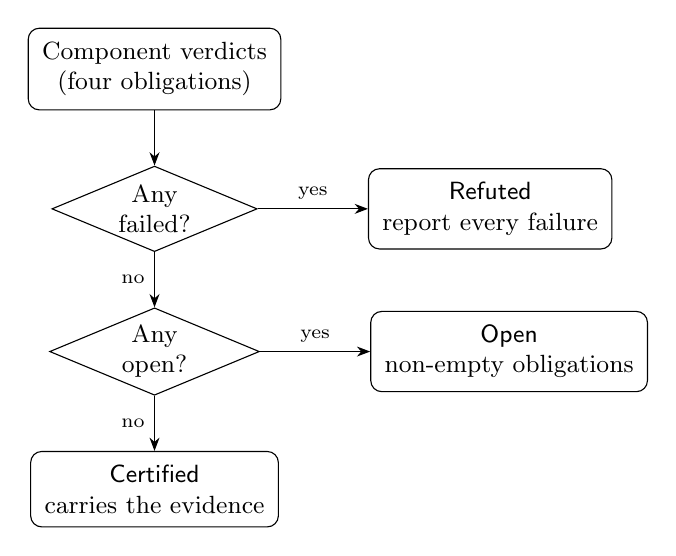
\begin{tikzpicture}[node distance=7mm and 14mm, box/.style={draw,rounded corners,align=center,inner sep=5pt,font=\small}, dia/.style={draw,diamond,aspect=2.4,align=center,inner sep=1pt,font=\small}, >=Stealth]
\node[box] (A) {Component verdicts\\ (four obligations)};
\node[dia,below=of A] (F) {Any\\ failed?};
\node[box,right=of F] (R) {$\Refu$\\ report every failure};
\node[dia,below=of F] (O) {Any\\ open?};
\node[box,right=of O] (U) {$\Open$\\ non-empty obligations};
\node[box,below=of O] (C) {$\Cert$\\ carries the evidence};
\draw[->] (A) -- (F);
\draw[->] (F) -- node[above,font=\scriptsize]{yes} (R);
\draw[->] (F) -- node[left,font=\scriptsize]{no} (O);
\draw[->] (O) -- node[above,font=\scriptsize]{yes} (U);
\draw[->] (O) -- node[left,font=\scriptsize]{no} (C);
\end{tikzpicture}
\caption{Verdict aggregation. The $\Refu$ value carries the located failures; the \emph{report} behind a verdict additionally retains every open and discharged obligation.}
\label{fig:aggregation}
\end{figure}

The distinction between report and verdict matters. If a failure co-occurs with an unresolved obligation the verdict is $\Refu$, but the unresolved obligation must not disappear merely because another obligation already refutes transport. It does not: it remains in the report. (In an earlier form of the development the assembled $\Refu$ value alone was the record, and dropped co-occurring open items; the report was introduced to repair this.)

\subsection{Assessment theorems}
The earlier work defines a transportability predicate $\mathsf{Transportable}$ with three \emph{abstract} propositional slots (exhibition, lineage grounding, functoriality); ``the'' legacy predicate is therefore a family. We use one instantiation and one strengthening, and keep them distinct:
\begin{align*}
\Tr_{\mathrm{leg}}(c) \;:\equiv\;{} & \mathsf{Inh}(\Sigma) \wedge \mathsf{Inh}(\mathsf{Exh}(c)) \wedge \mathsf{LineagePasses}(\ell) \wedge \Adm(M_A,\Phi_A)\\
& \wedge\ \Adm(M_B,\Phi_B) \wedge \mathsf{GE} \wedge \mathsf{Inh}(\mathrm{Mnt}),\\
\Tr(c) \;:\equiv\;{} & \Tr_{\mathrm{leg}}(c) \wedge \mathsf{Inh}(\mathrm{Aut}),
\end{align*}
where $\mathsf{Inh}(T) = \|T\|$. $\Tr_{\mathrm{leg}}(c)$ is the legacy predicate with its slots instantiated by inhabitation of the exhibition and maintenance evidence and by $\mathsf{LineagePasses}$. It contains no authority conjunct. $\Tr(c)$ adds one, and is therefore \emph{strictly stronger}: refuting $\Tr(c)$ does not in general refute $\Tr_{\mathrm{leg}}(c)$, because an authority failure refutes only the extra conjunct. The statements below are made at the correct level. \emph{(Coq: \coq{TransportableLegacy} for $\Tr_{\mathrm{leg}}$, \coq{TransportableFull} for $\Tr$; \coq{full_iff_legacy_and_authority}.)}

\begin{prop}[Certification soundness]\label{prop:certsound}
If $\mathsf{assemble}(v_1,\dots,v_4) = \Cert(\kappa)$ then $\kappa \in \mathsf{Cert}(c)$, $\Tr_{\mathrm{leg}}(c)$ holds, and $\Tr(c)$ holds. \emph{(Coq: \coq{certified_transportable_legacy}, \coq{certified_transportable}, \coq{certified_gives_transportable}.)}
\end{prop}
\begin{proof}
By \cref{def:assembly}, $\kappa$ is built from four discharged component verdicts, so $\kappa \in \mathsf{Cert}(c)$. Now read off each conjunct of $\Tr_{\mathrm{leg}}(c)$: $\mathsf{Inh}(\Sigma)$ from the inhabitant $\sigma_0$ of the construction certificate; $\mathsf{Inh}(\mathsf{Exh}(c))$ from its exhibition certificate; $\mathsf{LineagePasses}(\ell)$ because the lineage certificate has graph $\ell$ and carries proofs of well-formedness and L1--L3; the two admissibility conjuncts from the observation evidence; $\mathsf{GE}$ from the construction certificate; $\mathsf{Inh}(\mathrm{Mnt})$ from the maintenance evidence. The extra conjunct $\mathsf{Inh}(\mathrm{Aut})$ of $\Tr(c)$ comes from the authority evidence.
\end{proof}

\begin{prop}[Refutation soundness]\label{prop:refsound}
(a) Every \emph{non-institutional} located failure $f$ for $c$ refutes the legacy instantiation: $\neg\,\Tr_{\mathrm{leg}}(c)$, hence also $\neg\,\Tr(c)$.
(b) An \emph{institutional} (authority) failure refutes $\Tr(c)$, via the authority conjunct, and does not refute $\Tr_{\mathrm{leg}}(c)$.
(c) Consequently every located failure refutes $\Tr(c)$; if $\mathsf{assemble}(v_1,\dots,v_4) = \Refu(F)$ then $\neg\,\Tr(c)$ and $\mathsf{Cert}(c) = \emptyset$, and this holds of \emph{every} member of $F$. If moreover $F$ contains a non-institutional failure, then $\neg\,\Tr_{\mathrm{leg}}(c)$.
\emph{(Coq: \coq{located_refutes_legacy}, \coq{institutional_refutes_full}, \coq{located_refutes_transportable}, \coq{refuted_not_transportable}, \coq{located_refutes}, \coq{obstructions_refute}, \coq{each_obstruction_refutes}.)}
\end{prop}
\begin{proof}
(a) Assume $\Tr_{\mathrm{leg}}(c)$ and case on $f$ (\cref{tab:failures}). A fibre witness contradicts admissibility: if $\Phi = h \circ M$ and $M s_1 = M s_2$ then $\Phi s_1 = h(M s_1) = h(M s_2) = \Phi s_2$, contradicting $\Phi s_1 \neq \Phi s_2$. An empty seam contradicts $\mathsf{Inh}(\Sigma)$; a grounding failure at $r$ contradicts the grounding equation at $r$; a defeated exhibition contradicts $\mathsf{Inh}(\mathsf{Exh}(c))$; a coordinate-ground identity and a lineage descent contradict L1, and an undisclosed shared ancestor, the absence of an independent source, and a malformed record contradict, respectively, L2, L3 and well-formedness, all components of $\mathsf{LineagePasses}(\ell)$. A maintenance failure contradicts $\mathsf{Inh}(\mathrm{Mnt})$ by the refutation function of \cref{def:problem}. Since $\Tr(c)$ implies $\Tr_{\mathrm{leg}}(c)$, $\neg\Tr_{\mathrm{leg}}(c)$ gives $\neg\Tr(c)$.
(b) An authority failure contradicts $\mathsf{Inh}(\mathrm{Aut})$ by the refutation function of \cref{def:problem}, hence $\Tr(c)$. It says nothing about the conjuncts of $\Tr_{\mathrm{leg}}(c)$, none of which mentions authority; so this argument cannot refute the legacy predicate, and we do not claim it does.
(c) Combine (a) and (b). Since $\mathsf{Cert}(c)$ erases into $\Tr(c)$ by \cref{prop:certsound}, $\mathsf{Cert}(c) = \emptyset$. The final clauses apply (a) to a non-institutional member of $F$.
\end{proof}

\begin{prop}[Open non-emptiness and status characterisation]\label{prop:open}
$\mathsf{assemble}(v_1,\dots,v_4)$ is $\Open(D)$ iff no component is $\mathsf{Failed}$ and at least one is $\mathsf{Unresolved}$; then $D \neq [\,]$, and $D$ names exactly the unresolved obligations. It is $\Cert$ iff every component is $\mathsf{Discharged}$, and $\Refu$ iff some component is $\mathsf{Failed}$. \emph{(Coq: \coq{assemble_status}, \coq{assemble_open_nonempty}.)}
\end{prop}
\begin{proof}
By \cref{def:assembly} the first case applies iff $\mathsf{failures} \neq [\,]$, iff some component is $\mathsf{Failed}$. Otherwise no component is $\mathsf{Failed}$, so each of the four is $\mathsf{Discharged}$ or $\mathsf{Unresolved}$; if all are $\mathsf{Discharged}$ the second case applies, and otherwise some component is $\mathsf{Unresolved}$, so $D = \mathsf{opens}$ contains it and $D \neq [\,]$. The naming claim is the definition of $\mathsf{opens}$.
\end{proof}
An open assessment neither asserts transportability nor its negation.

\begin{prop}[Cumulative failure reporting]\label{prop:accumulate}
If $\mathsf{assemble}(v_1,\dots,v_4) = \Refu(F)$ then $F$ contains, in the fixed order observation, construction, maintenance, institution, the located failure of \emph{every} failed component and nothing else. Moreover the report accounts for each obligation exactly once: $|\mathsf{failures}| + |\mathsf{opens}| + |\mathsf{discharged}| = 4$, and the verdict of the report equals that of the assembled assessment. \emph{(Coq: \coq{assemble_refuted_reports_all}, \coq{report_accounts_for_all}, \coq{report_verdict_agrees}.)}
\end{prop}
\begin{proof}
$F = \mathsf{failures}$ is the concatenation, in order, of four lists, the $i$-th of which is the singleton $[f_i]$ if $v_i = \mathsf{Failed}(f_i)$ and empty otherwise. Each $v_i$ is exactly one of $\mathsf{Discharged}$, $\mathsf{Failed}$, $\mathsf{Unresolved}$, so it contributes one element to exactly one of the three lists, giving total length $4$. The verdict of the report is $\Refu$ when $\mathsf{failures} \neq [\,]$, else $\Open$ when $\mathsf{opens} \neq [\,]$, else $\Cert$, which is the case split of \cref{def:assembly}.
\end{proof}
Assessment is therefore \emph{cumulative} rather than precedence-based. Two examples in the development show this. A model with a copied ground \emph{and} a lost grounding fails two obligations, and both obstructions are reported, in order (\coq{both_obstructions_reported}). A model with a copied ground and maintenance not yet assessed has verdict $\Refu$ with one failure, and the unresolved maintenance obligation remains in the report (\coq{refuted_verdict_keeps_open_item}).

\subsection{Decidability}
Assembly is a total function once component verdicts have been supplied. That does not make the underlying obligations decidable: arbitrary admissibility is not generally decidable; lineage is decidable for the finite declared graph (\cref{sec:lineage}); institutional adequacy depends on supplied records and policies; and missing evidence yields $\Open$. When every obligation \emph{is} decidable, the open case disappears: the status is never $\Open$, $\Cert$ holds exactly when the conjunction of the obligations does, and $\Refu$ exactly when it does not (\coq{decidable_not_underdetermined}, \coq{decided_certified_iff_transport}, \coq{decided_refuted_iff_not_transport}). A Boolean classifier is thereby a \emph{specialisation} of the evidence-sensitive assessment, not its foundation.

\subsection{Interpretation}
The four obligations are diagnostic loci, not a partition: failures can and do coexist, which is why reports are cumulative. In the author's earlier manuscript they are called construction, observational, maintenance and institutional \emph{Warrant Debt} \cite{moore2026}; we use that vocabulary only here. The distinction between construction and maintenance is temporal and evidential: a ground that was never independently constituted is a construction failure; a ground that was valid at issuance and later ceased to agree is a maintenance failure. When the issuance record is absent, the causal classification may itself be unresolved.

\section{Certified lineage checking}\label{sec:lineage}

Lineage certificates (\cref{def:certs}) require a decision about a declared graph. This section defines that decision as a function, proves it correct, and shows that acceptance constructs a certificate.

\subsection{Finite lineage data}
\begin{defi}[Lineage record]\label{def:lineage}
A \emph{lineage record} $g$ is finite data: a list $D$ of pairs $(n,\mathit{ps})$ (a derived field and its parents); a list $\mathit{Raw}$ of raw inputs; a list $\mathit{Rel}$ of claim-relevant inputs; three distinguished nodes $d_A$, $d_B$ and $\gamma$ (the determinations $\Phi_A\circ\back$, $\Phi_B\circ\fwd$ and $\Phi_\Sigma$); and a list $\Delta$ of pairs $(n,\delta)$ giving a disposition (justified, or open defeater) to a shared ancestor. Nodes are natural numbers. Write $\mathsf{nodes}(g) = \mathsf{dom}(D) \mathbin{+\!\!+} \mathit{Raw}$, $N = |\mathsf{nodes}(g)|$, and $\mathsf{parents}_g(n)$ for the parents in the first entry of $D$ with key $n$ ($[\,]$ if none). A \emph{coverage record} is $\varkappa = (\mathsf{from},\mathsf{to},\mathsf{gaps})$ with $\mathsf{gaps}$ a list of unrecorded segments.
\end{defi}
$\mathrm{Anc}_g(n,m)$ (``$m$ is a strict ancestor of $n$'') is the least relation with $\mathrm{Anc}_g(n,m)$ whenever $m \in \mathsf{parents}_g(n)$, and $\mathrm{Anc}_g(n,m)$ whenever $p \in \mathsf{parents}_g(n)$ and $\mathrm{Anc}_g(p,m)$.

\begin{defi}[Lineage conditions]\label{def:L}
$\mathsf{WF}(g)$ holds iff: (1) $\mathsf{nodes}(g)$ is duplicate-free; (2) every parent of every entry is in $\mathsf{nodes}(g)$; (3) $d_A,d_B \in \mathsf{dom}(D)$ and $\gamma \in \mathsf{nodes}(g)$; (4) $\mathit{Rel} \subseteq \mathit{Raw}$; (5) $\neg\mathrm{Anc}_g(n,n)$ for all $n$. Further:
\begin{description}
\item[L1] (no identity, no descent) $\gamma \neq d_A$, $\gamma \neq d_B$, $\neg\mathrm{Anc}_g(\gamma,d_A)$ and $\neg\mathrm{Anc}_g(\gamma,d_B)$;
\item[L2] (disclosure) every $n$ with $\mathrm{Anc}_g(d_A,n)$, $\mathrm{Anc}_g(d_B,n)$ and $n \notin \mathit{Raw}$ lies in $\mathsf{dom}(\Delta)$;
\item[L3] (independent source) some $n \in \mathit{Raw} \cap \mathit{Rel}$ has $n = \gamma$ or $\mathrm{Anc}_g(\gamma,n)$, $\neg\mathrm{Anc}_g(d_A,n)$, $\neg\mathrm{Anc}_g(d_B,n)$, $n \neq d_A$, $n \neq d_B$.
\end{description}
$\mathsf{LineagePasses}(g) :\equiv \mathsf{WF}(g) \wedge \mathrm{L1} \wedge \mathrm{L2} \wedge \mathrm{L3}$.
\end{defi}
\paragraph{Status of L1--L3.} These conditions are \emph{declared specifications}, not derived results. They formalise three intelligible requirements on what it means for a seam valuation to be grounded independently of the coordinates it grounds: it must be neither one of them nor descended from them (L1), any ancestry it shares with them must be disclosed (L2), and it must draw on at least one claim-relevant source, possibly itself, that they do not (L3). We do not prove that they are necessary or sufficient for every adequate notion of grounding, and a different regime could adopt different conditions. What is proved is what the calculus needs of them: the copy pattern of \cref{sec:example} violates L1, and the checker below decides exactly these conditions.

\paragraph{Coordinates and ground.} Clause (3) of $\mathsf{WF}$ requires the coordinates $d_A$ and $d_B$ to be derived but requires the ground $\gamma$ only to be a declared node, so a raw input may serve as the ground. L3 accordingly ranges over $\gamma$ together with its strict ancestors, so that such a ground can be its own independent source. The identity clauses of L1 are not redundant: $\mathrm{Anc}_g$ is strict, and irreflexive under clause (5), so without them a ground equal to $d_A$ or $d_B$ would pass the descent test.

A passing verdict applies only to the declared graph \emph{and} its declared coverage: a partial record must not be reported as globally lineage-grounded. In the running example the ground $\gamma$ of the copied graph descends from $d_A$, so it violates L1.

\subsection{Ancestor saturation}
Ancestors are computed by saturation. Let $\mathsf{close}(S) = \mathsf{dedup}\bigl(S \mathbin{+\!\!+} \bigcup_{p \in S} \mathsf{parents}_g(p)\bigr)$ and, for a node $n$,
\[
S_0 = \mathsf{dedup}(\mathsf{parents}_g(n)), \qquad S_{k+1} = \mathsf{close}(S_k), \qquad \mathsf{anc}_g(n) = S_N .
\]
\begin{thm}[Ancestor correctness]\label{thm:anc}
(a) For every $g$: $m \in \mathsf{anc}_g(n) \Rightarrow \mathrm{Anc}_g(n,m)$.
(b) If every parent is declared ($\mathsf{(P)}$: $q \in \mathsf{parents}_g(p) \Rightarrow q \in \mathsf{nodes}(g)$), then $\mathrm{Anc}_g(n,m) \Rightarrow m \in \mathsf{anc}_g(n)$.
Hence under $(\mathsf{P})$, $m \in \mathsf{anc}_g(n) \Leftrightarrow \mathrm{Anc}_g(n,m)$. \emph{(Coq: \coq{ancestors_sound}, \coq{ancestors_complete}, \coq{ancestors_iff}.)}
\end{thm}
\begin{proof}
\emph{(a)} By induction on $k$, every element of $S_k$ is an ancestor of $n$. For $S_0$ this is the base clause of $\mathrm{Anc}$. If $m \in S_{k+1}$ then either $m \in S_k$, or $m \in \mathsf{parents}_g(p)$ for some $p \in S_k$; by hypothesis $\mathrm{Anc}_g(n,p)$, and appending a parent to an ancestor chain gives $\mathrm{Anc}_g(n,m)$.

\emph{(b)} Assume $(\mathsf{P})$ and fix $n$. We show that $S_N$ contains $n$'s parents and is closed under parents, and then that it contains every ancestor. Write $|S|$ for the length of a duplicate-free list.
\begin{enumerate}
\item[(i)] \emph{Monotone, duplicate-free, bounded.} $S_k \subseteq S_{k+1}$ (as $\mathsf{close}$ keeps $S_k$), each $S_k$ is duplicate-free (it is $\mathsf{dedup}$ of something), and $S_k \subseteq \mathsf{nodes}(g)$ by $(\mathsf{P})$ and induction on $k$. Hence $|S_k| \le N$ for all $k$.
\item[(ii)] \emph{Stabilisation propagates.} If $S_{k+1} \subseteq S_k$ then $S_{k+j} \subseteq S_k$ for all $j$. By induction on $j$: if $S_{k+j} \subseteq S_k$ then every parent of a member of $S_{k+j}$ is a parent of a member of $S_k$, hence lies in $S_{k+1} \subseteq S_k$; so $S_{k+j+1} = \mathsf{close}(S_{k+j}) \subseteq S_k$.
\item[(iii)] \emph{Non-stabilisation forces growth.} If $S_{i+1} \not\subseteq S_i$ for every $i < j$, then $|S_j| \ge j$. Each such step adds an element $x \notin S_i$ while keeping $S_i$; as $S_i$ is duplicate-free, $x :: S_i$ is duplicate-free and contained in $S_{i+1}$, so $|S_{i+1}| \ge |S_i| + 1$.
\item[(iv)] \emph{Stabilisation occurs by round $N$.} If $S_{i+1} \not\subseteq S_i$ for all $i \le N$, then (iii) with $j = N+1$ gives $|S_{N+1}| \ge N+1$, contradicting (i). So some $i \le N$ has $S_{i+1} \subseteq S_i$.
\item[(v)] \emph{$S_N$ is closed under parents.} With $i$ from (iv), (ii) gives $S_{N+1} \subseteq S_i \subseteq S_N$ (using monotonicity for $i \le N$). If $p \in S_N$ then $\mathsf{parents}_g(p) \subseteq S_{N+1} \subseteq S_N$.
\item[(vi)] \emph{Every ancestor is found.} We prove by induction on the derivation of $\mathrm{Anc}_g(a,m)$ that $(a = n \lor a \in S_N) \Rightarrow m \in S_N$. If $m \in \mathsf{parents}_g(a)$: for $a = n$, $m \in S_0 \subseteq S_N$; for $a \in S_N$ use (v). If $p \in \mathsf{parents}_g(a)$ and $\mathrm{Anc}_g(p,m)$: as before $p \in S_N$, and the induction hypothesis at $p$ gives $m \in S_N$. Taking $a = n$ gives the claim.\qedhere
\end{enumerate}
\end{proof}
The pigeonhole content is (iii)--(iv): a saturation that kept discovering new nodes after $N+1$ rounds would hold $N+1$ distinct declared nodes, more than the graph contains. The bound $N$ is used in the definition of $\mathsf{anc}_g$; only $(\mathsf{P})$ is needed, not acyclicity, which is itself checked below.

\subsection{Reflected conditions}
Define the Boolean checks: $\mathsf{wf}_1,\dots,\mathsf{wf}_4$ (clauses (1)--(4) of $\mathsf{WF}$, by list computation), $\mathsf{cycle}(g) = $ the first $n \in \mathsf{nodes}(g)$ with $n \in \mathsf{anc}_g(n)$; $\mathsf{c}_1$: $\gamma \neq d_A$, $\gamma \neq d_B$ and $d_A,d_B \notin \mathsf{anc}_g(\gamma)$; $\mathsf{c}_2$: every $n \in \mathsf{anc}_g(d_A)$ with $n \in \mathsf{anc}_g(d_B)$ and $n \notin \mathit{Raw}$ is in $\mathsf{dom}(\Delta)$; $\mathsf{c}_3$: some $n \in \{\gamma\} \cup \mathsf{anc}_g(\gamma)$ has $n \in \mathit{Raw} \cap \mathit{Rel}$, $n \notin \mathsf{anc}_g(d_A) \cup \mathsf{anc}_g(d_B)$, $n \neq d_A, d_B$.
\begin{lem}[Reflection of the conditions]\label{lem:reflect}
Each $\mathsf{wf}_i$ reflects clause $(i)$ of $\mathsf{WF}$, $i \le 4$. Under $(\mathsf{P})$, $\mathsf{c}_1 \Leftrightarrow \mathrm{L1}$, $\mathsf{c}_2 \Leftrightarrow \mathrm{L2}$ and $\mathsf{c}_3 \Leftrightarrow \mathrm{L3}$. \emph{(Coq: \coq{wf_defect_none_iff}, \coq{check_L1_reflect}, \coq{undisclosed_none_iff}, \coq{check_L3_reflect}.)}
\end{lem}
\begin{proof}
The first four are direct list facts (membership and duplicate-freedom are decided by traversal). For the rest, replace $\mathsf{anc}_g$ by $\mathrm{Anc}_g$ using \cref{thm:anc} (both directions, under $(\mathsf{P})$); the identity tests of $\mathsf{c}_1$ are equalities of natural numbers, and membership in $\{\gamma\} \cup \mathsf{anc}_g(\gamma)$ becomes $n = \gamma \lor \mathrm{Anc}_g(\gamma,n)$. Each check then states its condition verbatim.
\end{proof}

\subsection{Unconditional reflection}
The audit returns the first defect found, in the order: well-formedness (duplicate, undeclared parent, coordinate not derived or ground not declared, relevant input not raw, cycle), then L1 (ground equal to $d_A$, then to $d_B$, then descent from $d_A$, then from $d_B$), L2 (undisclosed shared ancestor), L3 (no independent source). Let $\mathsf{defect}(g) \in \mathsf{Option}(\text{Defect})$ be this result. Then
\[
\mathsf{lineageCheck}(g,\varkappa) \;=\;
\begin{cases}
\mathsf{Rejected}(d) & \text{if } \mathsf{defect}(g) = \mathsf{Some}(d),\\
\mathsf{Accepted} & \text{if } \mathsf{defect}(g) = \mathsf{None} \text{ and } \mathsf{gaps}(\varkappa) = [\,],\\
\mathsf{Open}(\mathsf{gaps}(\varkappa)) & \text{if } \mathsf{defect}(g) = \mathsf{None} \text{ and } \mathsf{gaps}(\varkappa) \neq [\,].
\end{cases}
\]
\begin{lem}\label{lem:defectnone}
$\mathsf{defect}(g) = \mathsf{None} \Longleftrightarrow \mathsf{LineagePasses}(g)$. \emph{(Coq: \coq{lineage_defect_none_iff}.)}
\end{lem}
\begin{proof}
($\Leftarrow$) Assume $\mathsf{LineagePasses}(g)$. By \cref{lem:reflect}, $\mathsf{wf}_1,\dots,\mathsf{wf}_4$ pass. If $\mathsf{cycle}(g) = \mathsf{Some}(n)$ then $n \in \mathsf{anc}_g(n)$, so $\mathrm{Anc}_g(n,n)$ by \cref{thm:anc}(a), contradicting clause (5). So no well-formedness defect is reported. Clause (2) is $(\mathsf{P})$, so by \cref{lem:reflect} the checks $\mathsf{c}_1,\mathsf{c}_2,\mathsf{c}_3$ pass, and no defect is reported at all.
($\Rightarrow$) Assume no defect. Then $\mathsf{wf}_1,\dots,\mathsf{wf}_4$ pass, giving clauses (1)--(4), in particular $(\mathsf{P})$. For clause (5) suppose $\mathrm{Anc}_g(n,n)$. Then $n$ has a parent, so $n$ is a key of $D$ and $n \in \mathsf{nodes}(g)$; by \cref{thm:anc}(b) $n \in \mathsf{anc}_g(n)$, so $\mathsf{cycle}(g)$ would report a cycle, a contradiction. So $\mathsf{WF}(g)$ holds. Now $(\mathsf{P})$ and passing $\mathsf{c}_1,\mathsf{c}_2,\mathsf{c}_3$ give L1, L2, L3 by \cref{lem:reflect}.
\end{proof}
\begin{thm}[Lineage-check reflection]\label{thm:reflect}
Unconditionally,
\[
\mathsf{lineageCheck}(g,\varkappa) = \mathsf{Accepted} \;\Longleftrightarrow\; \mathsf{LineagePasses}(g) \wedge \mathsf{gaps}(\varkappa) = [\,].
\]
\emph{(Coq: \coq{lineage_check_reflect}.)}
\end{thm}
\begin{proof}
$\mathsf{lineageCheck}(g,\varkappa) = \mathsf{Accepted}$ iff $\mathsf{defect}(g) = \mathsf{None}$ and $\mathsf{gaps}(\varkappa) = [\,]$; apply \cref{lem:defectnone}.
\end{proof}
The theorem needs no well-formedness hypothesis, unlike the conditional form one might first expect, because well-formedness is itself checked and reflected; soundness and completeness of ancestors (\cref{thm:anc}) are what make the acyclicity clause reflect.

\subsection{Rejected and open outcomes}
\begin{prop}[Rejection evidence]\label{prop:rejection}
If $\mathsf{lineageCheck}(g,\varkappa) = \mathsf{Rejected}(d)$ then the specification is violated in the way $d$ says, and $\neg\,\mathsf{LineagePasses}(g)$: a duplicate node, an undeclared parent, a coordinate that is not derived or a ground that is not a declared node, or a non-raw relevant input violates the corresponding clause of $\mathsf{WF}$; $\mathsf{Cycle}(n)$ gives $\mathrm{Anc}_g(n,n)$; $\mathsf{GroundEqualsA}$ (resp.\ $B$) gives $\gamma = d_A$ (resp.\ $\gamma = d_B$); $\mathsf{DescentFromA}$ (resp.\ $B$) gives $\mathrm{Anc}_g(\gamma,d_A)$ (resp.\ $d_B$); $\mathsf{UndisclosedShared}(n)$ gives $\mathrm{Anc}_g(d_A,n) \wedge \mathrm{Anc}_g(d_B,n) \wedge n \notin \mathit{Raw} \wedge n \notin \mathsf{dom}(\Delta)$; $\mathsf{NoIndependentSource}$ gives $\neg\mathrm{L3}$. \emph{(Coq: \coq{defect_sound}, \coq{lineage_check_rejected}.)}
\end{prop}
\begin{proof}
Each defect is produced by exactly one failed check in a fixed order; \cref{lem:reflect} and \cref{thm:anc} convert the failed check into the stated fact. For $\mathsf{Cycle}(n)$: $n \in \mathsf{anc}_g(n)$ and \cref{thm:anc}(a). The identity defects are equalities of node numbers. For descent and undisclosed ancestors, the same, since these are reported only after $\mathsf{WF}$ (hence $(\mathsf{P})$) has been established.
\end{proof}
\begin{prop}[Open outcomes]\label{prop:openlineage}
$\mathsf{lineageCheck}(g,\varkappa) = \mathsf{Open}(\mathit{gs})$ iff $\mathsf{LineagePasses}(g)$, $\mathsf{gaps}(\varkappa) = \mathit{gs}$ and $\mathit{gs} \neq [\,]$. In particular a defect takes precedence over a coverage gap. \emph{(Coq: \coq{lineage_check_open}.)}
\end{prop}
\begin{proof}
By the case split above and \cref{lem:defectnone}.
\end{proof}
Rejection therefore carries a located, specification-valid defect, while open means that the lineage conditions pass but declared coverage gaps remain.

\subsection{Certificate issuance}
\begin{thm}[Certificate issuance]\label{thm:issue}
There is a function $\mathsf{issue}(g,\varkappa) \in \mathsf{Option}(\mathsf{Lin})$ such that $\mathsf{issue}(g,\varkappa) = \mathsf{Some}(\lambda)$ iff $\mathsf{lineageCheck}(g,\varkappa) = \mathsf{Accepted}$, and then $\lambda$ has graph $g$, coverage $\varkappa$, and verdict $\mathsf{Pass}$. \emph{(Coq: \coq{issue_certificate}, \coq{issue_certificate_iff}, \coq{issue_certificate_data}.)}
\end{thm}
\begin{proof}
Define $\mathsf{issue}$ by cases on $\mathsf{defect}(g)$ and $\mathsf{gaps}(\varkappa)$; in the accepting case build the record from $g$, $\varkappa$, the verdict $\mathsf{Pass}$, and the proofs of $\mathsf{WF}$, L1, L2, L3 supplied by \cref{lem:defectnone} and the empty gaps. The iff is \cref{thm:reflect}.
\end{proof}
Acceptance thus constructs a kernel-checked certificate. This is strictly stronger than an audit that prints a verdict: the extracted checker returns a value whose type records that the graph passes.

\subsection{Pairwise audits do not compose}\label{sec:noncompose}
For a fixed lineage graph and fixed ground, L1 composes across consecutive coordinate pairs. L2 and L3 do not compose in general. Pairwise accepted lineage audits therefore do not certify the outer coordinate pair.

To state this without a composition operator on lineage records, fix every field of a record $g$ except the coordinates, and write $g[a,b]$ for $g$ with $d_A := a$ and $d_B := b$. The graph, the raw and claim-relevant inputs, the dispositions and the ground $\gamma$ are then the same in $g[A,B]$, $g[B,C]$ and $g[A,C]$, and so is $\mathrm{Anc}_g$, which depends only on $D$.

\begin{prop}[Fixed-graph, fixed-ground composition of L1]\label{prop:l1compose}
For every record $g$ and nodes $A,B,C$: if $g[A,B]$ and $g[B,C]$ satisfy L1, then so does $g[A,C]$. \emph{(Coq: \coq{L1_at_composes}.)}
\end{prop}
\begin{proof}
L1 for $g[a,b]$ is the conjunction of $\gamma \neq a$, $\neg\mathrm{Anc}_g(\gamma,a)$, $\gamma \neq b$ and $\neg\mathrm{Anc}_g(\gamma,b)$. The two clauses for $A$ come from $g[A,B]$ and the two for $C$ from $g[B,C]$.
\end{proof}
No well-formedness hypothesis is used. The statement fixes the ground: it says nothing about a composite whose ground, or whose graph, differs from those of the local audits.

\begin{prop}[L2 and L3 need not compose]\label{prop:noncompose}
There are records $g_2$ and $g_3$, and nodes $A,B,C$ for each, such that $\mathsf{LineagePasses}(g_i[A,B])$ and $\mathsf{LineagePasses}(g_i[B,C])$ hold for $i = 2,3$, while $g_2[A,C]$ is well-formed and satisfies L1 and L3 but not L2, and $g_3[A,C]$ is well-formed and satisfies L1 and L2 but not L3. \emph{(Coq: \coq{disclosure_noncomposition}, \coq{source_noncomposition}.)}
\end{prop}
\begin{proof}
Neither record has dispositions. Write $\mathsf{anc}(n)$ for the set of strict ancestors of $n$.

In $g_2$ the raw inputs are $0,1,2,3$, with $3$ claim-relevant; the derived fields are $4$ with parent $0$, $5$ and $7$ with parent $4$, $6$ with parent $1$, and the ground $8$ with parent $3$; take $(A,B,C) = (5,6,7)$. Then $\mathsf{anc}(5) = \mathsf{anc}(7) = \{0,4\}$, $\mathsf{anc}(6) = \{1\}$ and $\mathsf{anc}(8) = \{3\}$. The ground differs from and descends from no coordinate, $3$ witnesses L3 for every pair, and the pairs $(5,6)$ and $(6,7)$ share no ancestor, so both consecutive records pass. The outer pair $(5,7)$ shares the non-raw ancestor $4$, which has no disposition, so L2 fails, while L1 and L3 hold as before.

In $g_3$ the raw inputs are $0,1,2$, with $0$ and $1$ claim-relevant; the derived fields are $3$ with parent $1$, $4$ with parent $2$, $5$ with parent $0$, and the ground $6$ with parents $0$ and $1$; take $(A,B,C) = (3,4,5)$. No two coordinates share an ancestor, so L2 holds for every pair, and the ground differs from and descends from no coordinate, so L1 holds for every pair. For $(3,4)$ the input $0$ witnesses L3, and for $(4,5)$ the input $1$ does. For $(3,5)$ the only claim-relevant raw ancestors of the ground are $0$ and $1$, with $1 \in \mathsf{anc}(3)$ and $0 \in \mathsf{anc}(5)$, and the ground itself is not raw, so L3 fails.

Well-formedness of the six records, and the checker's verdicts (accepted for the consecutive pairs; $\mathsf{UndisclosedShared}(4)$ and $\mathsf{NoIndependentSource}$ for the two outer pairs), are established by computation and \cref{thm:reflect}.
\end{proof}

\begin{cor}[Fresh outer audit]\label{cor:freshaudit}
In general, lineage certificates for $g[A,B]$ and $g[B,C]$ do not yield one for $g[A,C]$: for the records of \cref{prop:noncompose}, the first two exist and the third does not. A lineage certificate for the outer pair therefore requires a fresh audit of that pair.
\end{cor}
\begin{proof}
A lineage certificate carries proofs of well-formedness and L1--L3 for its graph (\cref{def:certs}), so none exists for $g_i[A,C]$. For the consecutive records, with empty gaps, \cref{thm:issue} issues one.
\end{proof}
Composition of witnesses (\cref{thm:refl}) stays within one transport problem, and so under one lineage record. The outer pair $g[A,C]$ is a different record, which is why it needs its own audit.

\subsection{What the reflection theorem does not prove}
It proves equivalence between the Coq checker and the Coq specification. It does \emph{not} prove that the extracted checker agrees with an arbitrary handwritten implementation at the source-language semantic level; extraction remains within the stated trust boundary, and agreement with a handwritten audit is evidence of a different kind (\cref{sec:mechanisation}). Nor does it show that the declared graph contains every real production path.

\section{Mechanisation and regression evidence}\label{sec:mechanisation}

\subsection{Verified build}
The development is in Coq 8.18.0 \cite{coq818} and comprises roughly three and a half thousand lines of theory and nine hundred of examples. It builds with \texttt{coq\_makefile} and with \texttt{dune build}; \texttt{coqchk} succeeds on the whole project excluding one isolated file; and \texttt{Print Assumptions} reports each of the 120 Coq identifiers cited in this paper (92 of them in the ledger of \cref{app:ledger}) as closed under the global context. The one exception by design is the unrestricted functional converse of fibre factorisation, which needs classical choice and is confined to a single file that nothing else imports. Its constructive replacements are the relational form and, for finite domains with decidable equality, a direct construction. The main dependency closure is therefore axiom-free. \Cref{tab:trust} summarises the trust boundary.
\begin{table}[t]
\centering\small
\caption{Trust boundary and non-claims.}\label{tab:trust}
\begin{tabularx}{\textwidth}{@{}lY@{}}
\toprule
Checked mechanically & the theorems of this paper, in the Coq kernel; axiom-freeness of the main closure. \\
Trusted & the Coq kernel and extraction mechanism; the encoding of $\nat$ as OCaml integers in extracted code; the declared records themselves. \\
Tested, not proved & agreement of the extracted lineage audit with a handwritten audit (\cref{sec:regression}). \\
Not established & completeness of declared lineage; accuracy of raw inputs; adequacy of the state model; legitimacy or competence of an authority; decidability of general obligations. \\
\bottomrule
\end{tabularx}
\end{table}

\subsection{Legacy compatibility}
An earlier supplement (\cref{sec:seams}) is imported unchanged and built as an independent library. Its files match their recorded checksums, its own build-and-check procedure completes, and compatibility theorems recover its results from the generic calculus. Nothing in the earlier development was redefined.

\subsection{Extraction}\label{sec:extraction}
Certificate data live in $\Type$; their proofs live beside them. Extraction removes the proof fields and keeps the data (\cref{tab:survive}).
\begin{table}[t]
\centering\small
\caption{Evidence fields and whether they survive extraction.}\label{tab:survive}
\begin{tabularx}{\textwidth}{@{}lYc@{}}
\toprule
Component & Field & Survives \\
\midrule
Exhibition certificate & record id, identifiers, process, retained record and evaluator, coverage, custodian & yes \\
 & injectivity of identifiers; valuation factorisation & no \\
Lineage certificate & graph, coverage record with gaps, issued verdict & yes \\
 & well-formedness, L1--L3 & no \\
Construction certificate & seam inhabitant & yes \\
 & grounding equations & no \\
Obstruction & constructor tag; located data (seam element, node id) & yes \\
 & proofs (e.g.\ ancestor derivations) & no \\
Assessment & verdict, open reasons, gaps & yes \\
Maintenance and authority evidence & application-supplied data, via the summary interface & if in $\Type$ \\
\bottomrule
\end{tabularx}
\end{table}
We extracted the assessments of the examples to OCaml and wrote a consumer. For a certified assessment it reports the custodian (7), record identifier (1), lineage ground node (5) and audit verdict (\texttt{LineagePass}). For the copied model it reports a refutation at construction whose constructor names a lineage descent; for the maintenance model, a maintenance obstruction; for the model with both, both, in order; for missing and partial lineage records, an open assessment. The formal distinction thus survives compilation. It is materially stronger than attaching abstract propositions (\texttt{Exhibited}, \texttt{LineageGrounded}) to an ordinary relation, whose proofs would be erased.

Maintenance and authority evidence remain abstract types in the generic library. The generic calculus provides a \emph{summary interface}, a class assigning to each evidence type a function into a list of small extractable atoms (records, custodians, ground nodes, intervals, authorities, maintenance events, expiry, revalidation). Applications supply instances, so an extracted consumer can inspect more than the exhibition and lineage components without the kernel fixing an institutional schema. This is an observability extension, not a kernel correctness matter.

\subsection{Regression against a handwritten audit}\label{sec:regression}
The extracted checker (\cref{sec:lineage}) was compared with a handwritten OCaml lineage audit, by capturing the latter's printed output for the same records. This is \emph{differential regression testing}, not a proof of equivalence of the OCaml sources.

\paragraph{Case study.}
On five case-study records (live rows; backfill with a disclosed shared ancestor; backfill with it undisclosed; a copied seam valuation; a cyclic record) the two agree on all five, including the malformed cycle.

\paragraph{Unrestricted random records.}
On 3000 random records, including every malformation kind, they agree on all 3000. Only 89 of these were grounded, 1403 not grounded, 1508 malformed; the random population exercises the rejecting paths much more than the accepting path.

\paragraph{Stratified populations.}
To remedy this, we generate separate populations, each with a known \emph{intended} outcome. A graph passes only if (i) the extracted checker's verdict matches the intent, and (ii) its L1--L3 flags match the handwritten audit's output. The eleven \emph{shallow} populations, of 300 graphs each, are: accepted graphs (with random shared ancestry, dispositions and shuffled order); the same graphs with a coverage gap, intended $\mathsf{Open}$; one family for each single defect (descent from $d_A$, descent from $d_B$, undisclosed shared ancestor, no independent source); and one for each malformation (duplicate name, undeclared parent, distinguished node not derived, relevant input not raw, cycle). The handwritten audit has no notion of coverage, so the open population is checked against the intent and against the handwritten flags on the underlying graph.

\paragraph{Deep-ancestry populations.}
The mutation study below showed that the shallow populations are too shallow: their ancestor chains are short, so a saturation that stops early still finds every decisive ancestor. We therefore added six \emph{deep} populations of 300 graphs, in which the decisive ancestor is reachable only after several saturation rounds: the ground reaches its independent raw source through a chain of three to five derived nodes (depth at least four); descent from $d_A$ or $d_B$ is through a three-node branch (depth four); a shared derived ancestor is reached through chains of two to four nodes from each coordinate. The six populations are: accepted (L3 source at depth $\ge 4$), the same with a coverage gap ($\mathsf{Open}$), deep descent from $d_A$, deep descent from $d_B$, deep undisclosed shared ancestor, and deep no-independent-source. Together the seventeen populations comprise 5100 graphs, and all pass both criteria.

\paragraph{Mutation study.}
A test is only as good as its ability to fail. We textually mutated the \emph{extracted} checker in thirteen ways and recorded which suite detects each (\cref{tab:mutants}): the five-record case study (fixed), the unrestricted random population, the eleven shallow stratified populations, and the six deep populations.
\begin{table}[t]
\centering\small
\caption{Mutation study of the extracted lineage checker: $\times$ means the suite detects the mutant.}\label{tab:mutants}
\begin{tabular}{@{}lcccc@{}}
\toprule
Mutant & fixed & random & shallow & deep \\
\midrule
M1 drop the $d_B$ descent test (L1) & & $\times$ & $\times$ & $\times$ \\
M2 ignore dispositions (L2) & $\times$ & $\times$ & $\times$ & $\times$ \\
M3 raw shared ancestors count as undisclosed (L2) & $\times$ & $\times$ & $\times$ & $\times$ \\
M4 source need not be claim-relevant (L3) & & $\times$ & $\times$ & $\times$ \\
M5 source may be an ancestor of $d_A$ (L3) & & $\times$ & $\times$ & \\
M6 coverage gaps ignored & & & $\times$ & $\times$ \\
M7 skip relevance-is-raw check (WF) & & $\times$ & $\times$ & \\
M8 skip cycle detection (WF) & $\times$ & $\times$ & $\times$ & \\
M9 skip distinguished-derived check (WF) & & $\times$ & $\times$ & \\
M10 skip declared-parents check (WF) & & $\times$ & $\times$ & \\
M11 ancestors: parents only & $\times$ & $\times$ & $\times$ & $\times$ \\
M12 ancestors: one saturation step & $\times$ & $\times$ & & $\times$ \\
M13 ancestors: two saturation steps & & $\times$ & & $\times$ \\
\midrule
Mutants detected (of 13) & 5 & 12 & 11 & 8 \\
\bottomrule
\end{tabular}
\end{table}
All thirteen mutants are detected by the union of the suites, and by the stratified suite (shallow and deep together) alone. The individual suites are not equivalent, which is the argument for stratification. The random population detects twelve but misses M6, since the handwritten audit has no coverage; M6 is caught only by the open populations. The shallow populations detect eleven, and \emph{miss} the bounded-saturation mutants M12 and M13, because their graphs are shallow; the unrestricted random population detected those two because it happens to generate deeper graphs; and the deep populations, added in response, detect both. The fixed case study detects five and would not have found, for instance, the dropped $d_B$ descent test (M1).

The theorem of \cref{sec:lineage} already establishes checker correctness. These tests probe extraction, the encoding of records, the differential harness, and diagnostic agreement with the handwritten implementation; the mutation study measures whether that probe can fail.

\section{Related work}\label{sec:related}

We do not claim that proof relevance, provenance, labelled transitions or certified transformation are new. The contribution is a calculus that combines witness-bearing rewriting with lineage conditions, coverage, cumulative obstruction reporting and open assessment, together with the erasure results that relate it to ordinary rewriting. For each neighbouring formalism we ask what evidential structure it retains and what grounded transport adds or refuses to erase.

\paragraph{Generalised rewriting and \texttt{Proper} (Sozeau).}
Generalised rewriting in Coq \cite{sozeau2009} lets a rewrite step be justified by a relation and by \texttt{Proper} (respectful) instances, resolved by type-class search; relations and their proofs are propositions. A rewriting step therefore yields a proof term, but relatedness itself is an indistinguishable proposition, so the way it was established is not data an extracted program can inspect. Grounded transport keeps this framework as its extensional image: erasure returns an ordinary preorder (\cref{prop:preorder}) and certificate-proper and crossing-proper contexts erase to \texttt{Proper} instances (\cref{thm:twolevels}). What it adds is a type-valued judgement whose inhabitants are distinguishable (\cref{thm:multiplicity}) and a notion of context that maps witnesses. It also drops symmetry: transport is directed, and the erased relation is a preorder, not necessarily a setoid.

\paragraph{Proof-relevant logical relations (Benton, Hofmann, Nigam).}
Proof-relevant logical relations \cite{benton2014} equip relations with witnesses of relatedness that can be composed, so that relatedness records how it was established; they are used to justify effect-dependent program transformations. The shared idea is that a relation should carry evidence. The purpose differs: their witnesses are semantic and internal to a proof about programs, whereas ours record externally declared process evidence (seam, exhibition record, lineage, coverage, authority), are assessed against conditions that can fail or remain unresolved, and are designed to survive extraction. We do not claim that proof-relevant relations are new, and we do not prove effect-based transformation results.

\paragraph{Groupoid interpretations and non-trivial proof identity (Hofmann, Streicher).}
The groupoid model shows that identity proofs need not be unique \cite{hofmann1994,hofmann1998}: distinct proofs of the same equation can be distinguished. Distinguishable witnesses between the same endpoints are the same phenomenon in our setting (\cref{thm:multiplicity}). But our structure is directed and free, is a category only up to the crossing-sequence equivalence (\cref{thm:algebra}), has no inverses, and makes no claim about identity types or higher structure. What we add is not higher homotopy but an account of \emph{which} extractable data distinguish witnesses, and of what erasure forgets.

\paragraph{Provenance semirings (Green, Karvounarakis, Tannen).}
Provenance semirings \cite{green2007} annotate tuples with elements of a commutative semiring and propagate the annotations through positive relational algebra, retaining, in the universal case, a polynomial describing how each tuple was derived; the survey \cite{cheney2009} places this beside why- and where-provenance \cite{buneman2001}. This retains the multiplicity and structure of derivations. Conditions L1--L3 concern something else: which derivations a ground \emph{may not} share with the coordinates it is meant to ground, and whether shared ancestry has been disclosed. That is a property of a declared derivation graph relative to a claim, not an annotation of a query result. The two are complementary: an algebraic provenance computation could supply the lineage record that our checker (\cref{sec:lineage}) then judges. We do not provide algebraic propagation.

\paragraph{W3C PROV}
PROV-DM \cite{prov2013} standardises descriptive provenance: entities, activities and agents, and relations such as derivation and attribution. It records what is asserted to have happened, and deliberately does not say when a record licenses a claim. Our lineage record is comparable to a derivation graph, but grounded transport adds checkable conditions on it (independence of the ground, disclosure of shared ancestry, a claim-relevant source), declared coverage with gaps, and an assessment that keeps missing evidence distinct from counterevidence. A mapping from PROV documents to lineage records is future work and would be a way to obtain the records our checker consumes.

\paragraph{Proof-carrying code and certified transformation.}
Proof-carrying code \cite{necula1997} ships code with a machine-checkable proof; verified compilers \cite{leroy2009} prove semantic preservation once and for all; translation validation \cite{pnueli1998} checks each compilation run instead. All carry or check evidence that a transformation preserves semantics or safety. Grounded transport carries evidence about a different question: whether an agreement between representations is independently grounded, how it was produced, over what coverage, and with which obligations unresolved. Its per-problem certificate is closest in spirit to translation validation (a per-instance check) but its assessments admit a third outcome, $\Open$, for obligations that no available procedure decides.

\paragraph{Rewriting logic, transition systems, categories.}
Rewriting logic \cite{meseguer1992} and labelled transition systems retain transition labels; a label alone need not contain checkable lineage, coverage and warrant evidence, and grounded witnesses can be read as richly certified labels, a reading we do not develop. The categorical structure of witnesses \cite{maclane1998} is the one described above, up to $\weq$.

\paragraph{Factorisation, assurance.}
The obstruction results build on the standard criterion that a predicate factors through an observation exactly when it is constant on its fibres, in the manner of the exactness condition of abstract interpretation \cite{cousot1977}; we use it as an established tool. The certified/refuted/open distinction supports assurance arguments that must retain defeaters and unresolved obligations rather than issue only success or failure \cite{bloomfield2020}.

\begin{table}[t]
\centering\small
\caption{What each neighbour retains, and what grounded transport adds.}\label{tab:related}
\begin{tabularx}{\textwidth}{@{}lYY@{}}
\toprule
Neighbour & Retains & Grounded transport adds (or refuses to erase) \\
\midrule
Generalised rewriting & relation, \texttt{Proper} instances (as propositions) & type-valued witnesses; witness-mapping contexts; directedness \\
Proof-relevant logical relations & semantic witnesses of relatedness & externally declared process evidence; failure and open states; extraction \\
Groupoid model & non-unique identity proofs & which extractable data distinguish witnesses; two-stage erasure \\
Provenance semirings & multiplicity and structure of derivations & claim-relative independence conditions L1--L3; coverage \\
W3C PROV & descriptive derivation records & checkable conditions on such records; assessment \\
PCC, verified compilation, translation validation & semantic-preservation evidence & grounding, lineage, authority; an $\Open$ outcome \\
\bottomrule
\end{tabularx}
\end{table}

\section{Discussion and limitations}\label{sec:limitations}

\subsection{Processual motivation}\label{sec:whitehead}
The calculus was motivated by a reading of process philosophy in which settled endpoints correspond to coordinate description, while the transition that produced them has a character that endpoint agreement does not exhaust \cite{whitehead1929}. The formal calculus does not encode any ontology and should not be read as doing so. It formalises one methodological consequence: \emph{endpoint agreement does not exhaust the evidence relevant to a processual transition}. The fuller philosophical treatment, including a taxonomy of warrant obligations, is in an earlier manuscript by the author \cite{moore2026}. The results of this paper stand on the need to retain process and provenance evidence, and do not depend on accepting that metaphysics.

\subsection{Limitations}
\paragraph{Declared-graph limitation.}
A lineage certificate proves properties of the \emph{declared} graph. It does not prove that the graph contains every real production path, and the audit cannot detect a path the record omits.

\paragraph{Raw inputs and state models.}
The calculus can identify claim-relevant raw inputs without proving that they accurately record the concrete process, and cannot show that the state model adequately represents the target.

\paragraph{Institutional limitation.}
Authority and custodianship can be represented as data, but their legitimacy and competence are not established internally; the rule system is an input. Exhibition conditions concerning the declared process, coverage and custodian are recorded, not verified.

\paragraph{Decidability.}
General transport obligations need not be decidable; the open assessment is essential, not an implementation inconvenience.

\paragraph{Coverage.}
Preservation on the image of an evolution does not certify new target states outside that image (\cref{thm:coverage}).

\paragraph{Certificate-level preservation needs an evidence lift.}
Seam evolutions are crossing-proper given preservation of grounding on the image. They are certificate-proper only under an evidence lift (\cref{def:pm}), which we supply by reissuing certificates in one model and show cannot exist in another (\cref{thm:reissue}). A general theory of maintaining exhibition records, lineage and coverage across evolutions, rather than reissuing them, is not developed (\cref{rem:crossinglevel}).

\paragraph{Witness algebra and composition.}
Identity and associativity hold up to the crossing-sequence equivalence, not by literal equality (\cref{thm:algebra}). In a single seam, composition of non-identity crossing witnesses is degenerate (\cref{rem:degenerate}).

\paragraph{The endpoint theorem is extensional.}
The equality concluded by seam transport needs only extensional agreement; grounding strengthens its warrant, not its algebraic conclusion (\cref{sec:seams}).

\paragraph{The audit boundary.}
The Coq checker is proved to reflect its specification; the handwritten OCaml audit is tested against it, not proved equivalent (\cref{sec:regression}), and its decision core has not been replaced by the extracted checker. The stratified test graphs are shallow (\cref{tab:mutants}, M12).

\paragraph{Scope of the model.}
Valuations are Boolean; a general value space with a value transport is used only in the statement of valuation naturality. Maintenance and authority evidence are abstract. No rewriting tactic is provided, and no empirical claim is made: the examples are separating models showing that distinctions are real, not evidence of usability or scalability on production systems.

\section{Conclusion}\label{sec:conclusion}

The central distinction is between
\[
\text{same endpoint judgement} \;\neq\; \text{same warrant}.
\]
Grounded transport carries evidence; composition and contexts preserve it, at the level of crossings always and at the level of complete certificates when an evidence lift exists; erasure yields ordinary substitutability and loses information irreversibly; observational agreement cannot license lineage-sensitive substitution, and located obstructions explain failed transport; open assessments preserve unresolved obligations, and a refutation does not discard them; a finite lineage audit is proved to reflect its specification and, once extracted, issues certificates; and extraction retains the evidential data that downstream audits require.

Ordinary rewriting answers whether one expression may replace another under a relation. Grounded transport additionally answers through which process, under which lineage, within what coverage, and with which remaining obligations that replacement is warranted. Erasure recovers ordinary substitutability, but ordinary substitutability cannot reconstruct the warrant that was erased.

The calculus does not make declarations true. It makes precisely explicit what has been declared, checks what can be checked, and reports what has not been resolved. Witness-carrying rewriting tactics, and a treatment of certificates carried along evolutions, are natural next steps that rest on the semantics established here.


\bibliographystyle{alphaurl}
\bibliography{refs}

\appendix
\section{Theorem ledger and proof status}\label{app:ledger}

Each row names the Coq identifier(s) of a result of the paper. \emph{Proof in paper} says whether the proof is given in full (\textbf{F}), summarised (\textbf{S}), or omitted (\textbf{M}, mechanised only). Every omitted or summarised proof is mechanised in the artefact, and every identifier below was checked to exist and to be closed under the global context, except where noted.

{\small
\begin{longtable}{@{}r>{\raggedright\arraybackslash}p{3.7cm}>{\raggedright\arraybackslash}p{5.4cm}>{\raggedright\arraybackslash}p{2.0cm}c@{}}
\caption{Theorem spine and its mechanisation.}\label{tab:ledger}\\
\toprule
\# & Result & Coq identifier(s) & Text & Proof \\
\midrule
\endfirsthead
\toprule
\# & Result & Coq identifier(s) & Text & Proof \\
\midrule
\endhead
\bottomrule
\endfoot
1 & Grounded reflexivity, composition & \coq{grounded_transport_refl}, \coq{grounded_transport_compose} & \cref{thm:refl} & S \\
2 & Witness algebra modulo $\weq$ & \coq{WEquiv_id_left}, \coq{WEquiv_id_right}, \coq{WEquiv_assoc}, \coq{WEquiv_compose}, \coq{WEquiv_summary} & \cref{thm:algebra} & F \\
3 & Erasure soundness & \coq{erase_sound}, \coq{rpath_sound}, \coq{erasure_sound} & \cref{thm:soundness} & F \\
4 & Erased preorder & \coq{erased_PreOrder} & \cref{prop:preorder} & S \\
4$'$ & Exact recovery under completeness & \coq{erasure_exact_of_complete}, \coq{preorder_complete}, \coq{not_complete_of_gap} & \cref{prop:complete} & M \\
5 & Erasure non-reflection & \coq{erasure_not_reflecting}, \coq{copied_ungrounded_agreement} & \cref{thm:nonreflect} & F \\
6 & Same endpoints, different warrants & \coq{packed_warrants_same_endpoints}, \coq{same_endpoints_different_warrants}, \coq{packed_distinguishable} & \cref{thm:multiplicity} & F \\
6$'$ & Observational obstruction & \coq{fibre_obstruction}, \coq{not_proper_of_distinguished}, \coq{observational_not_grounded}, \coq{obs_equiv_not_transport}, \coq{trace_not_determined_by_copied_value} & \cref{prop:obsobstruction} & F \\
7 & Composition of witness-preserving contexts & \coq{gp_id}, \coq{gp_comp}, \coq{grounded_proper_compose} & \cref{thm:gpcomp} & F \\
8 & Two levels: composition, chain, nesting & \coq{crossing_proper_id}, \coq{crossing_proper_comp}, \coq{certificate_proper_id}, \coq{certificate_proper_comp}, \coq{certificate_proper_erased}, \coq{crossing_proper_erased}, \coq{contextual_chain}, \coq{contextual_preservation}, \coq{contextual_preservation_nested}, \coq{grounded_proper_erased}, \coq{grounded_proper_Proper}, \coq{grounded_proper_sound} & \cref{thm:twolevels} & F \\
8$'$ & Evidence lifting gives certificate-proper & \coq{pm_certificate_proper}, \coq{pm_crossing_proper}, \coq{pm_commute}, \coq{lift_gives_grounding} & \cref{thm:lifting} & F \\
9 & Grounding erases to pairwise agreement & \coq{original_grounding_erases_to_extensional} & \cref{prop:groundingerases} & F \\
10 & Pairwise agreement $\not\Rightarrow$ grounding & \coq{pairwise_agreement_not_grounding}, \coq{copied_extensionally_coherent}, \coq{copied_not_grounded} & \cref{prop:pairwise} & F \\
11 & Original seam transport recovered & \coq{original_seam_transport_from_generic}, \coq{extensional_factor_transport}, \coq{grounded_factor_transport} & \cref{thm:seamtransport,prop:extfactor,cor:groundedfactor} & F \\
12 & Dynamic separation & \coq{dynamic_failure_visible}, \coq{ordinary_rewriting_still_succeeds}, \coq{structural_naturality_not_preservation} & \cref{thm:dynfail} & F \\
12$'$ & Naturality preserves grounding on image & \coq{natural_valuations_preserve_grounding_on_image}, \coq{grounding_at_transported_elements} & \cref{thm:preserve} & F \\
12$''$ & Global preservation under coverage & \coq{surjective_evolution_preserves_all_grounding}, \coq{preservation_without_coverage} & \cref{thm:coverage} & F \\
12$'''$ & Certificate reissue; no lift when grounding lost & \coq{reissue_certificate_proper}, \coq{no_evidence_lift_when_grounding_lost}, \coq{evolution_crossing_proper} & \cref{thm:reissue} & F \\
13 & Certification soundness & \coq{certified_transportable_legacy}, \coq{certified_transportable}, \coq{certified_gives_transportable}, \coq{full_iff_legacy_and_authority}, \coq{full_implies_legacy} & \cref{prop:certsound} & F \\
14 & Refutation soundness (legacy and full) & \coq{located_refutes_legacy}, \coq{institutional_refutes_full}, \coq{located_refutes_transportable}, \coq{refuted_not_transportable}, \coq{obstructions_refute}, \coq{each_obstruction_refutes} & \cref{prop:refsound} & F \\
15 & Open non-emptiness, status & \coq{assemble_status}, \coq{assemble_open_nonempty} & \cref{prop:open} & F \\
16 & Cumulative failure reporting & \coq{assemble_refuted_reports_all}, \coq{report_accounts_for_all}, \coq{report_verdict_agrees}, \coq{both_obstructions_reported}, \coq{refuted_verdict_keeps_open_item} & \cref{prop:accumulate} & F \\
17 & Ancestor saturation & \coq{ancestors_sound}, \coq{ancestors_complete}, \coq{ancestors_iff} & \cref{thm:anc} & F \\
17$'$ & Reflection of conditions & \coq{wf_defect_none_iff}, \coq{check_L1_reflect}, \coq{undisclosed_none_iff}, \coq{check_L3_reflect} & \cref{lem:reflect} & S \\
18 & Lineage-check reflection & \coq{lineage_defect_none_iff}, \coq{lineage_check_reflect} & \cref{lem:defectnone,thm:reflect} & F \\
19 & Rejection evidence, open outcomes & \coq{defect_sound}, \coq{lineage_check_rejected}, \coq{lineage_check_open} & \cref{prop:rejection,prop:openlineage} & S \\
20 & Certificate issuance & \coq{issue_certificate_iff}, \coq{issue_certificate_data} & \cref{thm:issue} & S \\
\midrule
--- & Functional converse of fibre factorisation (classical; \emph{not} axiom-free) & \coq{constant_factors} (isolated file) & \cref{sec:mechanisation} & M \\
\end{longtable}
}

\paragraph{Regression evidence (not theorems).}
The case-study, random, stratified and mutation results of \cref{sec:regression} are produced by the scripts in the artefact's extraction directory; they are tests and are not part of the ledger.


\end{document}
